\chapter{
MCMC for Spatial Capture-Recapture
}
\markboth{MCMC}{}
\label{chapt.mcmc}

%%% NOTES
%%% Andy's working through this doing format edits mostly and math
%%% stuff , but not in order
%%% anytime you see a XXX or XYZ that is a marker to change some
%%% hard-wired reference to a float

\vspace{.3in}

\section{Introduction}
In this chapter we will dive a little deeper into Markov chain Monte
Carlo (MCMC) sampling. We will construct custom MCMC samplers in {\bf R},
starting with easy-to-code GLMs and GLMMs and moving on to simple CR and SCR
models. Finally, we will illustrate some alternative
ready-to-use software packages for MCMC sampling. We will NOT provide
exhaustive background information on the theory and justification of
MCMC sampling -- there are entire books dedicated to that subject and
we refer you to \citet{robert_casella:2004} and
\citet{robert_casella:2010}. Rather we aim to provide you with enough
background and technical know-how to start building your own MCMC
samplers for SCR models in {\bf R}. You will find that quite a few topics that come up 
in this chapter have already been covered in previous chapters, particularly the introduction
into Bayesian analysis in Chapt. \ref{chapt.glms}. To keep you from having to leaf back and forth
we will in some places briefly review aspects of Bayesian analysis, but we try to focus on the more 
technical issues of building MCMC samplers relevant to SCR models. 



\subsection{Why build your own MCMC algorithm?}

The standard programs we have used so far to run MCMC analyses are
{\bf WinBUGS} \citep{gilks_etal:1994} and {\bf JAGS}
\citep{plummer:2003}. The wonderful thing about these {\bf BUGS}
engines
is that they automatically use  appropriate and, most of the time,
efficient forms
of MCMC sampling for the model specified by the user.

The fact that we have such a Swiss Army knife type of MCMC machine
begs the question: Why would anyone want to build their own MCMC
algorithm? For one, there are a limited number of distributions and
functions implemented in {\bf BUGS}. While {\bf OpenBUGS} provides more
options, some more complex models may be impossible to build within
these programs. A very simple example from spatial capture-recapture
that can give you a headache in {\bf WinBUGS} is when your state-space is an
irregular-shaped polygon, rather than an ideal rectangle that can be
characterized by four pairs of coordinates. It is easy to restrict
activity centers to any arbitrary polygon in {\bf R} using an ESRI shapefile
(and we will show you an example in a little bit), but you cannot use
a shape file in a {\bf BUGS} model.  Similarly, models of space usage
that take into account ecological distance
(Chapt. \ref{chapt.ecoldist}) cannot be implemented in the {\bf BUGS}
engines.  Moreover, there are classes of 
SCR models that we have not been able to implement effectively using
likelihood methods, and are inefficient to run in the {\bf BUGS}
engines. An example are those models covered in Chapts. 
\ref{chapt.scr-unmarked} and \ref{chapt.partialID}. 

Sometimes implementing an MCMC algorithm in R may be faster than in
{\bf WinBUGS} - especially if you want to run simulation studies where you
have hundreds or more simulated data sets, several years' worth of
data or other large models, this can be a big advantage.

Finally, building your own MCMC algorithm is a great exercise to
understand how MCMC sampling works. So while using the {\bf BUGS} language requires you to understand the structure of your model, building an MCMC algorithm requires you to think about the relationship between your data, priors and posteriors, and how these can be efficiently analyzed and characterized. Not to mention that, if you are an {\bf R} junkie, it can actually be fun.
However, if you don't think you will ever sit down and write your own
MCMC sampler, consider skipping this chapter - apart from coding it
will not cover anything SCR-related that is not covered by other, more
model-oriented chapters as well.


\section{MCMC and posterior distributions}

MCMC is a class of simulation methods for
drawing (correlated) random numbers from a target distribution, which
in Bayesian inference is the posterior distribution.
As a reminder, the posterior distribution is a probability
distribution for an unknown parameter, say $\theta$, given a set of
observed data and its prior probability distribution (the probability
distribution we assign to a parameter before we observe data).  The
great benefit of computing the posterior distribution of $\theta$ is
that it can be used to make probability statements about $\theta$,
such as the probability that $\theta$ is equal to some value, or the
probability that $\theta$ falls within some range of values. 
The posterior distribution summarizes all we know about a parameter
and thus, is the central object of interest in Bayesian
analysis. Unfortunately, in many if not most practical applications,
it is nearly impossible to directly compute the posterior. Recall
Bayes’ theorem:
\begin{equation}
[\theta|y] = \frac{[y|\theta] [\theta]}  {[y]},
\label{mcmc.eq.bayes}
\end{equation}
where $\theta$ is the parameter of interest, $y$ is the observed data,
$[\theta|y]$ is the posterior, $[y|\theta]$ the likelihood of the
data conditional on $\theta$, $[\theta]$ the prior probability of
$\theta$, and, finally, $[y]$ is the marginal probability of the
data, defined as 
\[
[y] = \int [y|\theta]  [\theta] d\theta
\]

This marginal probability is a normalizing constant that ensures that
the posterior integrates to 1. Often, the
integral is  hard or impossible to evaluate, unless you are
dealing with a really simple model.  For example, consider 
a Normal model, with a set of $n$ observations, $y_{i};
i=1,2,\ldots,n$: 
\[
 y_{i} \sim \mbox{Normal}(\mu, \sigma),
\]
where $\sigma$ is known and our objective is to obtain an estimate of
$\mu$ using Bayesian statistics. To fully specify the model in a Bayesian
framework, we first have to define a prior distribution for $\mu$. Recall
from Chapt. \ref{chapt.glms} 
that for certain data models, certain priors lead to
conjugacy, i.e. if you choose a certain prior for your parameter,
your posterior distribution will be of a known parametric form. The
conjugate prior for the mean of a Normal model is also a Normal
distribution:
\[
\mu \sim \mbox{Normal}(\mu_0, \sigma_{0}^{2})
\]
If $\mu_{0}$ and $\sigma_{0}^{2}$ are fixed, the posterior for $\mu$
has the following form (for some of the algebra behind this, see Chapt. 2 in \citet{gelman_etal:2004}):
\begin{equation}
\mu|y \sim \mbox{Normal}(\mu_{n}, \sigma_{n}^{2})
\label{mcmc.eq.mu-posterior}
\end{equation}
where
\[
\mu_{n} = \frac{ \sigma^{2}}  {\sigma^{2}   +n \sigma_{0}^{2}}*  \mu_0 +      \frac{n  \sigma_{0}^{2}}  {\sigma^{2}   +n \sigma_{0}^{2}} *\bar{y}
\]
And
\[
 \sigma_{n}^{2} = \frac{\sigma^{2}  \sigma_{0}^{2}} {\sigma^{2} + n \sigma_{0}^{2}}
\]
We can directly obtain estimates of interest from this Normal
posterior distribution, such as the mean $\hat{\mu}$ and its variance; we
do not need to apply MCMC, since we can recognize the posterior as a
parametric distribution, including the normalizing constant $[y]$.
But generally we will be interested in more complex models with
several, say $m$, parameters. In this case, computing $[y]$ from
Eq. \ref{mcmc.eq.bayes} requires $m$-dimensional integration, which is
can be difficult or impossible. Thus, the posterior distribution in
generally only known up to a constant of proportionality:
\[
[\theta|y] \propto [y|\theta] * [\theta]
\]
The power of MCMC is that it allows us to approximate the posterior
using simulation without evaluating the high dimensional integrals and
to directly sample from the posterior, even when the posterior
distribution is unknown! The price is that MCMC is computationally
expensive. Although MCMC first appeared in the scientific literature
in 1949 \citep{metropolis_etal:1949}, widespread use did not occur
until the 1980s when computational power and speed increased
\citep{gelfand_smith:1990}. It is safe to say that the advent of
practical MCMC methods is the primary reason why Bayesian inference
has become so popular during the past three decades.
In a nutshell, MCMC lets us generate sequential draws of $\theta$ (the
parameter(s) of interest) from distributions approximating the unknown
posterior over $T$ iterations. The distribution of the draw at $t$ depends
on the value drawn at $t$-1; hence, the draws from a Markov
chain\footnote{In case you are not familiar with Markov chains, for
  $T$ random samples $\theta^ {(1)}$, ... $\theta^{(T)}$ from a Markov chain
  the distribution of $\theta^{(t)}$ depends only on the immediately preceding
  value, $\theta^{(t-1)}$.}. As $T$ goes to infinity, the Markov chain
converges to the desired distribution – in our case the posterior
distribution for $\theta|y$. Thus, once the Markov chain has reached
its stationary distribution, the generated samples can be used to
characterize the posterior distribution, $[\theta|y]$, and point
estimates of $\theta$, its standard error and confidence bounds, can
be obtained directly from this approximation of the posterior. 



\section{Types of MCMC sampling}

There are several MCMC algorithms, the most popular being Gibbs
sampling and Metropolis-Hastings sampling, both of which were briefly introduced in Chapt. \ref{chapt.glms}. We will be dealing with
these two classes in more detail and use them to construct the MCMC
algorithms for SCR models. Also, we will briefly review alternative
techniques that are applicable in some situations.


\subsection{Gibbs sampling}
\label{mcmc.sec.gibbs}

Gibbs sampling was named after the physicist J.W. Gibbs by
\citet{geman_geman:1984}, who applied the algorithm to a Gibbs
distribution \footnote{a distribution from physics we are not going to
  worry about, since it has no immediate connection with Gibbs
  sampling other than giving its name}. The roots of Gibbs sampling
can be traced back to work of \citet{metropolis_ulam:1953}, and it is
actually closely related to Metropolis sampling (see Chapt. 11.5 in
\citet{gelman_etal:2004}, for the link between the two samplers). We
will focus on the technical aspects of this algorithm, but if you find
yourself hungry for more background, \citet{casella_george:1992}
provide a more in-depth introduction to the Gibbs sampler.

Let's go back to our
simple example from above to understand the motivation and functioning
of Gibbs sampling. Recall that for a Normal model with known variance
and a Normal prior for $\mu$, the posterior distribution of $\mu|y$ is also
Normal. Conversely, with a fixed (known) $\mu$, but unknown variance, the
conjugate prior for $\sigma^2$ is an Inverse-Gamma distribution with shape and scale parameters $a$ and $b$:
\[
\sigma^2 \sim InvGamma(a,b),
\]
With fixed $a$ and $b$, the posterior $[\sigma|\mu,y]$ is also an Inverse Gamma distribution, namely:
\begin{equation}
\sigma|\mu,y \sim InvGamma (a_n, b_n),
\label{eq. 3}
\end{equation}
XXXXX Andy, when do we use square brackets around $\theta|y$ and when don't we? On a similar note, when do we use the asterisk for multiplication? Any rules? XXXXXXX
 where  $a_n = n/2   + a$ and $b_n = (1/2) \displaystyle\sum\limits_{i=1}^{n} (y_i-\mu)^2 + b$.
However, what if we know neither $\mu$ nor $\sigma$, which is probably the
more common case? The joint posterior distribution of $\mu$ and $\sigma$
now has the general structure
\[
[\mu, \sigma|y] = \frac{[y|\mu] [\mu] [\sigma]}{ \int [y|\mu] [\mu] [\sigma] d\mu d\sigma }
\]
or
\[
[\mu, \sigma|y] \propto [y|\mu] [\mu] [\sigma]
\]
\begin{comment} Rahel : use of p() here might violate some convention of the
book -- I dunno. Lets think about it 
I changed it to the way you use in Ch2
\end{comment}
This cannot easily be reduced to a distribution we recognize. However,
we can condition $\mu$ on $\sigma$ (i.e., we treat $\sigma$ as fixed) and remove
all terms from the joint posterior distribution that do not involve $\mu$
to construct the full conditional distribution,
\[
[\mu|\sigma,y]  \propto [y|\mu] [\mu]
\]

The full conditional of $\mu$ again takes the form of the Normal
distribution shown in Eq. \ref{mcmc.eq.mu-posterior}; similarly, $[\sigma|\mu,y]$ takes
the form of the Inverse Gamma distribution shown in
Eq. \ref{eq. 3}, both distribution we can easily sample
from. And this is precisely what we do when using Gibbs sampling: we
break down high-dimensional problems into convenient one-dimensional
problems by constructing the full conditional distributions for each
model parameter separately; and we sample from these full
conditionals, which, if we choose conjugate priors, are known
parametric distributions.
Let's put the concept of Gibbs sampling into the MCMC framework of
generating successive samples, using our simple Normal model with
unknown $\mu$ and $\sigma$ and conjugate priors as an example. These are the
steps you need to build a Gibbs sampler:

{\flushleft {\bf Step 0:} Begin with some initial values for $\theta$, $\theta^{(0)}$.}
In our example, we have to specify initial values for $\mu$ and $\sigma$, for
example by drawing a random number from some Uniform distribution, or
by setting them close to what we think they might be. (Note: This step
is required in any MCMC sampling; chains have to start from
somewhere. We will get back to these technical details a little
later.)
{\flushleft {\bf Step 1:} Draw $\theta^{(1)}$ from the conditional distribution $[\theta_{1}^{(1)}|\theta_{2}^{(0)}$,\ldots, $\theta_{d}^{(0)}]$. }
Here, $\theta_1$ is $\mu$, which we draw from the Normal distribution in Eq. \ref{mcmc.eq.mu-posterior}  using $\sigma^{(0)}$ as value for $\sigma$.
{\flushleft {\bf Step 2:} Draw $\theta_{2}^{(1)}$ from the conditional distribution $[\theta_{2}^{(1)}|\theta_{1}^{(1)}$, $\theta_{3}^{(0)}$,\ldots, $\theta_{d}^{(0)}]$. }
Here, $\theta_2$ is $\sigma$, which we draw from the Inverse Gamma
distribution of Eq. \ref{eq. 3}, using $\mu^{(1)}$ as value for $\mu$.

{\flushleft {\bf Step 3:} Draw $\theta_{d}^{(1)}$ from the conditional distribution $[\theta_{d}^{(1)}|\theta_{1}^{(1)}$,\ldots, $\theta_{d-1}^{(1)}]$. }
In our example we have no additional parameters, so we only need step 0 through to 2.

{\flushleft Repeat Steps 1 to $d$ for $T$ = a large number of samples.}

In terms of {\bf R} coding, this means we have to write Gibbs updaters for
$\mu$ and $\sigma$ and embed them into a loop over $T$ iterations. The final
code in the form of an {\bf R} function is shown 
in Panel \ref{mcmc.panel.gibbs1}.


\begin{panel}[htp]
\centering
\rule[0.15in]{\textwidth}{.03in}
%\begin{minipage}{2.5in}
\begin{verbatim}
Norm.Gibbs<-function(y=y,mu_0=mu_0,sigma2_0=sigma2_0,a=a,b=b,niter=niter){

ybar<-mean(y)
n<-length(y)
mu<-1            #mean initial value
sigma2<-1        #sigma2 initial value
an<-n/2 + a      #shape parameter of IvGamma distribution of sigma2

out<-matrix(nrow=niter, ncol=2)
colnames(out)<-c('mu', 'sig')

for (i in 1:niter) {

#update mu according to Eq. 7.2
mu_n<- (sigma2/(sigma2+n*sigma2_0))*mu_0 + (n*sigma2_0/(sigma2 + n*sigma2_0))*ybar 
sigma2_n <- (sigma2*sigma2_0)/ (sigma2 + n*sigma2_0)
mu<-rnorm(1,mu_n, sqrt(sigma2_n))

#update sigma2 according to Eq. 7.3
bn<- 0.5 * (sum((y-mu)^2)) + b
sigma2<-1/rgamma(1,shape=an, rate=bn)
out[i,]<-c(mu,sqrt(sigma2))

}
return(out)
}
\end{verbatim}
%\end{minipage}
\rule[-0.15in]{\textwidth}{.03in}
\caption{
R-code for a Gibbs sampler for a Normal model with unknown $\mu$
and $\sigma$ and conjugate priors (Normal and Inverse Gamma, respectively) 
for both parameters.
}
\label{mcmc.panel.gibbs1}
\end{panel}

This is it! You can go ahead and simulate some data, $y \sim \mbox{Normal}(5, 0.5)$ and then use the function \mbox{\tt NormGibbs()} in the {\bf
  R} package \mbox{\tt scrbook} to run your first Gibbs sampler. 

\begin{verbatim}
set.seed(13)

#true mean and sd are 5 and 0.5
y<-rnorm(1000, 5,0.5) #data

mu_0<-0 #prior mean
sigma2_0<-100 #prior variance 

#InvGamma hyperparameters
a<-0.1
b<-0.1 

mod=Norm.Gibbs(y, mu_0, sigma2_0, a,b,niter=10000)
\end{verbatim}

Your output, \verb#mod#, will be a table with two columns, one per
parameter, and $T$ rows, one per iteration. For this 2-parameter example
you can visualize the joint posterior by plotting samples of $\mu$
against samples of $\sigma$ (Fig. \ref{postdist.fig}):
\begin{verbatim}
plot(out[,1], out[,2])
\end{verbatim}
The marginal distribution of each parameter is approximated by just
examining the samples of this particular parameter. You can visualize
it by plotting a histogram of the samples (Fig. \ref{plotsofPD.fig} upper left and right):
\begin{verbatim}
par(mfrow=c(1,2))
hist(out[,1]); hist (out[,2])
\end{verbatim}

Finally, recall an important characteristic of Markov chains, namely,
that the chain has to have converged (reached its stationary
distribution) in order to regard samples as coming from the posterior distribution. In
practice, that means you have to throw out some of the initial samples
– called the burn-in. We will talk about this in more when we talk
about convergence diagnostics. For now, you can use the
\verb#plot(out[,1])# or \verb#plot(out[,2])# command to make a time
series plot of the samples of each parameter and visually assess how
many of the initial samples you should discard. Fig. \ref{plotsofPD.fig} bottom left and right shows
plots for the estimates of $\mu$ and $\sigma$ from our simulated data set;
you see that in this simple example the Markov chain apparently
reaches its stationary distribution very quickly -- the chains look
'grassy' seemingly from the start. It is hard to discern a burn-in
phase visually (but we will see examples further on where the burn-in
is clearer) and you may just discard the first 500 draws to be sure
you only use samples from the posterior distribution. The mean of the
remaining samples are your estimates of $\mu$ and $\sigma$:
\begin{verbatim}
summary(mod[501:10000,])
       mu             sig        
 Min.   :4.935   Min.   :0.4652  
 1st Qu.:4.988   1st Qu.:0.4930  
 Median :4.998   Median :0.5006  
 Mean   :4.998   Mean   :0.5008  
 3rd Qu.:5.009   3rd Qu.:0.5084  
 Max.   :5.062   Max.   :0.5486  
\end{verbatim}

\begin{figure}
\begin{center}
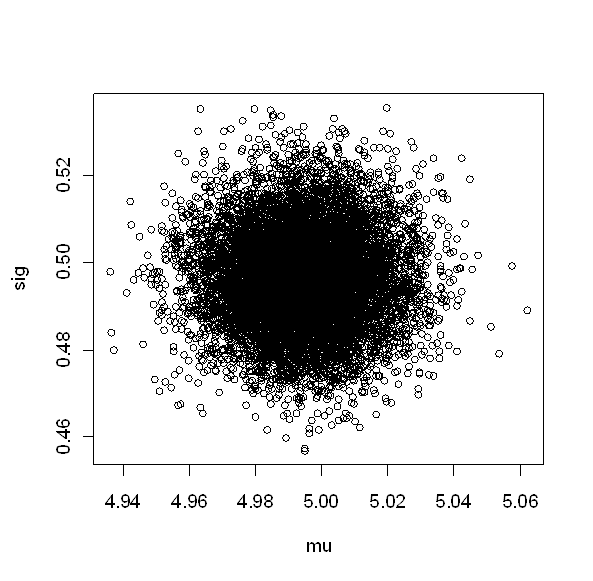
\includegraphics[height=4in]{Ch7/figs/postdist}
\end{center}
\caption{Joint posterior distribution of $\mu$ and $\sigma$ from a Normal Model}
\label{postdist.fig}
\end{figure}

\begin{figure}
\begin{center}
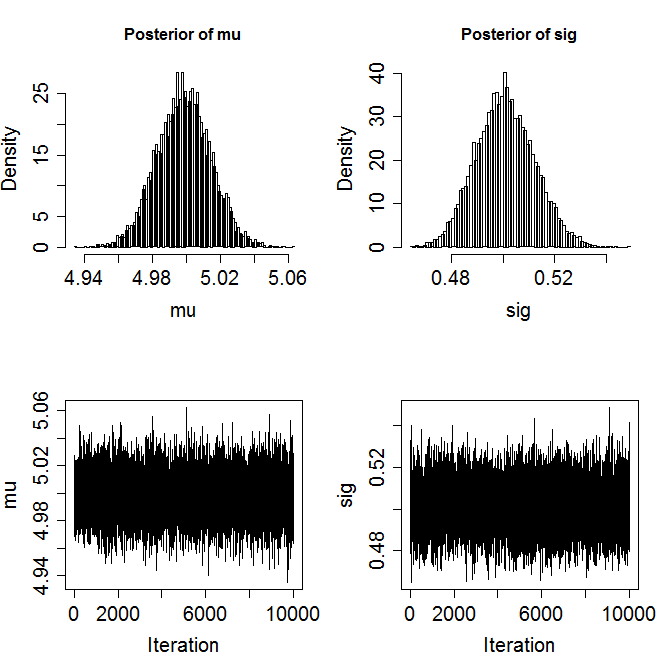
\includegraphics[width=5in]{Ch7/figs/plotsofPD}
\end{center}
\caption{
Plots of the posterior distributions of $\mu$ (upper left) and
  $\sigma$ (upper right)
  from a Normal model and time series plots of $\mu$ (lower left) and $\sigma$ (lower right).}
\label{plotsofPD.fig}
\end{figure}


\subsection{ Metropolis-Hastings sampling   }

Although it is applicable to a wide range of problems, the limitations
of Gibbs sampling are immediately obvious: what if we do not want to
use conjugate priors (or what if we cannot recognize the full
conditional distribution as a parametric distribution, or simply do
not want to worry about these issues)? The most general solution is to
use the Metropolis-Hastings (MH) algorithm, which also goes back to
the work by \citet{metropolis_ulam:1953}. You saw the basics of this
algorithm in Chapt. \ref{chapt.glms}. In a nutshell, because we do not recognize the
posterior $[\theta|y]$ as a parametric distribution, the MH algorithm
generates samples from a known proposal distribution, say $h(\theta)$,
that depends on $\theta$ at $t-1$. The $t^{th}$ sample is accepted with probability. 

\[
r = \frac{ [\theta^{(t-1)}|y] h(\theta^{(t)}|\theta^{(t-1)})}
    {[\theta^{(t)}|y] h(\theta^{(t-1)}|\theta^{(t)}) }
\]

Proposal distributions can be absolutely
anything!  You can generate candidate values from a $normal(0,1)$
distribution, from a uniform(-3455,3455) distribution, or anything of
proper support.  Note, however, that good choices of $h()$ are those
that approximate the posterior distribution. Obviously if $h() =
[\theta|y]$ (i.e., the posterior) then you always accept the draw,
and it stands to reason that proposals that are more similar to
$[\theta|y]$ will lead to higher acceptance probabilities. 

The original Metropolis algorithm
required $h(\theta)$ to be symmetric so that
$h(\theta^{(t)}|\theta^{(t-1)}) = h(\theta^{(t-1)}|\theta^{(t)})$. 
In that case these two terms just cancel
out from the MH acceptance probability and $r$ is then just the ratio
of the target density evaluated at the candidate value to that
evaluated at the current value. A later
development of the algorithm by \citet{hastings:1970} lifted this
condition. 
Since using a symmetric proposal distribution makes life a little
easier, we are going to focus on this specific case. A type of symmetric proposal useful in many situations is the
so-called {\it random-walk} proposal distribution where candidate values
are drawn from a normal distribution with mean equal to the current
value and some standard deviation, say $\delta$, which is prescribed by
the user (see below for further explanation). 

{\bf Parameters with bounded support}: Many models contain parameters that
have  bounded support. E.g., variance parameters live on $[0,\infty]$,
parameters that represent probabilities live on $[0,1]$, etc..
For such cases, it is sometimes convenient to use a random
walk proposal distribution that can generate any real number (e.g., a
normal random walk proposal). Under these circumstances you should not constrain the proposal distribution itself, 
but you can just reject parameters that are
outside of the parameter space \citep{robert_casella:2010}. You will see plenty of examples of updating parameters with bounded support in this chapter. 

It is worth
knowing that there are alternatives to the random walk MH algorithm. For
example, in the independent M-H, $\theta^{(t)}$ does not depend on
$\theta^{(t-1)}$, while the Langevin algorithm \citep{roberts_etal:1998}
aims at avoiding the random walk by favoring moves towards regions of
higher posterior probability density. The interested reader should
look up these algorithms in \citet{robert_casella:2004} or
\citet{robert_casella:2010}.

Building a MH sampler can be broken down into several steps. We are going to demonstrate these steps using a different but still simple and common model: the logit-normal or logistic regression model. For simplicity, assume that
\[
y \sim \mbox{Bern} \left(\frac{\exp(\theta)}{1+ \exp(\theta)}\right)
\]
and
\[
\theta \sim \mbox{Normal}(\mu, \sigma)
\]
The following steps are required to set up a random walk MH algorithm:

{\flushleft {\bf Step 0}: Choose initial values, $\theta^{(0)}$.}

{\flushleft {\bf Step 1}: Generate a proposed value of $\theta$ at $t$ from $h(\theta^{(t)}|\theta^{(t-1)})$. }
We often use a Normal proposal distribution, so we draw $\theta^{(1)}$ from $\mbox{Normal}(\theta^{(0)}, \delta)$, where $\delta$ is the variance of the Normal proposal distribution, the tuning parameter that we have to set.

{\flushleft {\bf Step 2}: Calculate the ratio of posterior densities for the proposed and the original value for $\theta$: }
\[
r = \frac{[\theta^{(t)}|y]}  {[\theta^{(t-1)}|y]}
\]
In our example,
\[
r = \frac{\mbox{Bern}(y|\theta^{(t)}) * \mbox{Normal}(\theta^{(t)}|\mu, \sigma)} {\mbox{Bern}(y|\theta^{(t-1)}) * \mbox{Normal}(\theta^{(t-1)}|\mu, \sigma)}
\]


{\bf Step 3}: Set
\begin{eqnarray*}
\theta^{(t)}  &= &   \theta^{(t)} \mbox{ with probability min(r,1)}\\
	 & = & 	\theta^{(t-1)} \mbox{ otherwise }
\end{eqnarray*}

%should work now


We can do that by drawing a random number $u$ from a
$\mbox{Unif}(0,1)$ and accept $\theta^{(t)}$ if
$u<r$.
Repeat for $t = 1,2,\ldots$ a large number of samples.
The {\bf R} code for this MH sampler is provided in Panel \ref{mcmc.panel.logitnormal}.

\begin{panel}[htp]
\centering
\rule[0.15in]{\textwidth}{.03in}
%\begin{minipage}{2.5in}
{\small
\begin{verbatim}
Logreg.MH<-function(y=y, mu0=mu0, sig0=sig0, delta=delta, niter=niter) {

out<-c()

theta<-runif(1, -3,3) #initial value

for (iter in 1:niter){
theta.cand<-rnorm(1, theta, delta)

loglike<-sum(dbinom(y, 1, exp(theta)/(1+exp(theta)), log=TRUE))
logprior <- dnorm(theta,mu0 ,sig0, log=TRUE)
loglike.cand<-sum(dbinom(y, 1, exp(theta.cand)/(1+exp(theta.cand)), log=TRUE))
logprior.cand <- dnorm(theta.cand, mu0, sig0, log=TRUE)

if (runif(1)<exp((loglike.cand+logprior.cand)-(loglike+logprior))){
theta<-theta.cand
}
out[iter]<-theta
}

return(out)
}
\end{verbatim}
}
%\end{minipage}
\rule[-0.15in]{\textwidth}{.03in}
\caption{
{\bf R} code to run a Metropolis sampler on a simple Logit-Normal model.
}
\label{mcmc.panel.logitnormal}
\end{panel}



The reason we sum the logs of the likelihood and the prior, rather than multiplying the original values, is simply computational. The product of small probabilities can be numbers very close to 0, which computers do not handle well. Thus we add the logarithms, sum, and exponentiate to achieve the desired result. Similarly, in case you have forgotten some elementary math, $x/y = exp(log(x)-log(y))$, with the latter being favored for computational reasons.

Comparing MH sampling to Gibbs sampling, where all draws from the
conditional distribution are used, in the MH algorithm we discard a
portion of the candidate values, which inherently makes in less
efficient than Gibbs sampling -- the price you pay for its increased
generality.  In Step 1 of the MH sampler we had to choose a variance,
$\delta$, for the Normal proposal distribution. Choice of the
parameters that define our candidate distribution is also referred to
as 'tuning', and it is important since adequate tuning will make your
algorithm more efficient.  $\delta$ should be chosen (a) large enough
so that each step of drawing a new proposal value for $\theta$ can
cover a reasonable distance in the parameter space, as otherwise,
mixing of the Markov chain is inefficient and chains will tend to have
strong autocorrelation; and (b) small enough so that proposal values
are not rejected too often, as otherwise the random walk will 'get
stuck' at specific values for too long.  As a rule of thumb, your
candidate value should be accepted in about 40\% of all
cases. Acceptance rates of 20 -- 80\% are probably ok, but anything
below or above may well render your algorithm inefficient (this does
not mean that it will give you wrong results, only that you will need
more iterations to converge to the posterior distribution). In
practice, tuning will require some 'trial-and-error', some common
sense and, with enough experience, some intuition. Or, one can use an adaptive phase, where the tuning parameter
is automatically adjusted until it reaches a user-defined acceptance
rate, at which point the adaptive phase ends and the actual Markov
chain begins. This is computationally a little more
advanced. \citet{link_barker:2009} discuss this in more detail. It is
important the samples drawn during the adaptive phase are discarded.
To illustrate the effects of tuning, we ran the
Metropolis-within-Gibbs algorithm in Panel \ref{mcmc.panel.logitnormal} with $\delta=0.01$,
$\delta=0.2$ and $\delta=1$. The first 150 iterations for $\theta$ are
shown in Fig. \ref{mcmc.fig.tuning}. We see that for a very small
$\delta$ (the dashed line) the burn-in is extremely slow - after 150
iterations the chain isn't even half way there, while for the other
two values of $\delta$ (solid and dotted)the burn-in phase seems to be
over after only about 10 iterations. While $\delta=0.2$ leads to
reasonably good mixing, the chain clearly gets stuck on certain values
with $\delta=1$.
%'tuning' is a new figure I made... don't know about the size specifications, just copied those from another picture. Do you set them at 
%the actual size of the figure or the size you want it to be??
 \begin{figure}
\begin{center}
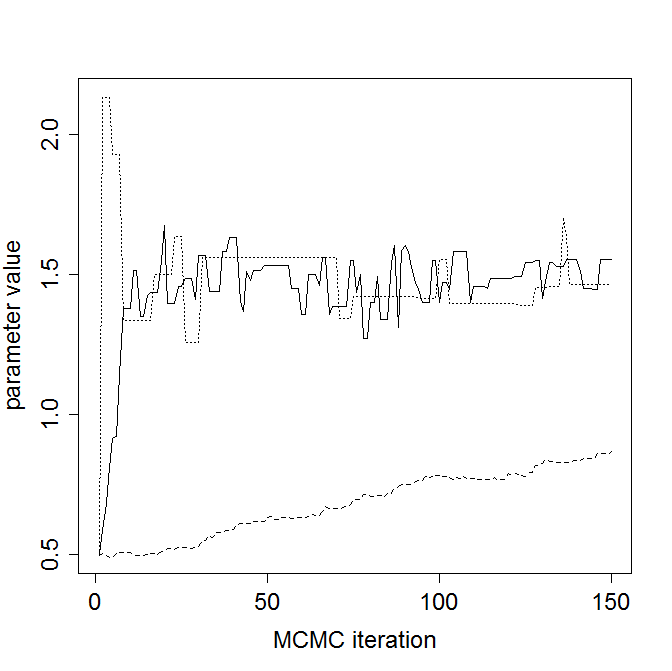
\includegraphics[height=3in,width=3.5in]{Ch7/figs/tuning}
\end{center}
\caption{Time series plots of $\theta$ from a MH algorithm with tuning parameter  $\delta = 0.01$ (dashed line), 0.2 (solid line) and  1 (dotted line).}
\label{mcmc.fig.tuning}
\end{figure}

Other than graphically, you can easily check acceptance rates for the parameters you monitor (that are part of your output) using the \verb#rejectionRate()# function of the package coda (we will talk more about this package a little later on). Do not let the term 'rejection rate' confuse you; it is simply 1 -- acceptance rate. There may be parameters -- for example, individual values of a random effect or latent variables -- that you do not want to save, though, and in our next example we will show you a way to monitor their acceptance rates with a few extra lines of code.



\subsection{ Metropolis-within-Gibbs }

One weakness of the MH sampler is that formulating the joint posterior when evaluating whether to accept or reject the candidate values for $\theta$ becomes increasingly complex or inefficient as the number of parameters in a model increases. As you already saw in Chapter 2, in these cases you can simply combine MH sampling and Gibbs sampling. You can use Gibbs sampling to break down your high-dimensional parameter space into easy-to-handle one-dimensional conditional distributions and use MH sampling for these conditional distributions. Better yet, if you have some conjugacy in your model, you can use the more efficient Gibbs sampling for these parameters and one-dimensional MH for all the others. You have already seen the basics of how to build both types of algorithms, so we can jump straight into an example here and build a Metropolis-within-Gibbs algorithm.

XXXX Maybe we make this an unnumbered subsubsection... since it's still part of the 'Types of MCMC samplers' section...
\subsubsection*{ GLMMs: Poisson regression with a random effect }

Let's assume a model that gets us closer to the problem we ultimately
want to deal with - a GLMM. Here, we assume we have Poisson counts,
$y_{ij}$, from $j=1,2,\ldots,n$ plots in $i$ different study sites, and we believe that the counts are influenced by some plot-specific covariate, ${\bf x}$, but that there is also a random site effect. So our model is:
\begin{comment} Rahel: I put
  ``n'' here because you had ``n'' used above. But I wonder if we
  should have a convention for ``number of sites'' and use that
  throughout the book?  I think we use j=1,..,J for traps .... I can't
  remember what I used in Ch. 2. but maybe i'm overthinking
  this. lets talk later. \end{comment} 
  
\[
y_{ij} \sim \mbox{Poisson}(\lambda_{ij})
\]
\[
\lambda_{ij} = \exp (\alpha_i + \beta x_{ij})
\]
Let's use Normal priors on $\alpha$ and $\beta$,  \[
\alpha_i \sim \mbox{Normal} (\mu_{\alpha}, \sigma_{\alpha})
\]
and
\[
\beta \sim \mbox{Normal} (\mu_{\beta}, \sigma_{\beta})
\].

Since we want to estimate the random effect on $\alpha$ in this model, we do not
specify $\mu_{\alpha}$ and $\sigma_{\alpha}$, but instead, estimate them as well, so we have
to specify hyperpriors for these parameters:
\begin{eqnarray*}
\mu_{\alpha}  &\sim &  \mbox{Norm}(\mu_0, \sigma_0)  \\
\sigma_{\alpha} & \sim & \mbox{InvGamma}(a_0, b_0)
\end{eqnarray*}
Note that for simplicity we assume that $\beta$ is constant across the $i$ study sites, and for analysis we would set $\mu_{\beta}$ and $\sigma_{\beta}$.
With the model completely specified, we can compile the full conditionals,
breaking the multi-dimensional parameter space into one-dimensional
components:

\begin{eqnarray*}
[\alpha_1|\alpha_2,\alpha_3,\ldots,\alpha_i,\beta,{\bf y}_{1}] & \propto &   [{\bf y}_{1}|\alpha_1,\beta] * [\alpha_1] \\
	 & \propto  &   \mbox{Poisson}({\bf y}_{1}| \exp(\alpha_1 + \beta {\bf x}_1)) * \mbox{Norm}(\alpha_1|\mu_{\alpha} , \sigma_{\alpha})
\end{eqnarray*}
where ${\bf y}_{1} = (y_{11},y_{12}, \ldots, y_{1n})$ is the vector of
observed counts for site $i=1$ and, in general, ${\bf y}_{i}$ is the
vector of all counts for site $i$; analogous,${\bf x}_{i}$ is the
vector of all observations of the covariate for site $i$. The other full conditionals for
each $\alpha_{i}$ are constructed similarly:
\begin{comment} 
Does it look right now?
\end{comment}
\begin{eqnarray*}
[\alpha_2|\alpha_1,\alpha_3,\ldots,\alpha_i,\beta,{\bf y}_{2}] & \propto&  [{\bf y}_{2}|\alpha_2,\beta] * [\alpha_2] \\
	 & \propto  & \mbox{Poisson}({\bf y}_{2}| \exp(\alpha_2 + \beta {\bf x}_2)) * \mbox{Norm}(\alpha_2|\mu_{\alpha}, \sigma_{\alpha})
\end{eqnarray*}
and so on for all elements of ${\bf \alpha}$. The full-conditional for $\beta$ is:
\begin{eqnarray*}
[\beta|\alpha,{\bf y}] &\propto & [{\bf y}|\alpha,\beta] * [\beta] \\
	 &\propto& \mbox{Poisson}({\bf y}|exp(\alpha + \beta {\bf x})) *\mbox{Norm}(\beta|\mu_{\beta}, \sigma_{\beta})
\end{eqnarray*}

Finally, we need to update the hyperparameters for the random effects
vector ${\bf \alpha}$:
\[
[\mu_{\alpha}|{\bf \alpha}] \propto [{\bf \alpha}|\mu_{\alpha}, \sigma_{\alpha}] *[\mu_{\alpha}]
\]
\[
[\sigma_{\alpha}|{\bf\alpha}] \propto [\alpha|\mu_{\alpha}, \sigma_{\alpha}] *[\sigma_{\alpha}]
\]
Since we assumed ${\bf \alpha}$ to come from a Normal distribution, the choice of priors for $\mu_{\alpha}$ (Normal) and $\sigma_{\alpha}$ (Inverse-Gamma) leads to the same conjugacy we observed in our initial Normal model, so that both hyperparameters can be updated using Gibbs sampling.

Now let's build the updating steps for these full conditionals. Again, for the MH steps that update ${\bf \alpha}$ and $\beta$ we use Normal proposal distributions with standard deviations $\delta_{\alpha}$ and $\delta_{\beta}$.

First, we set the initial values ${\bf \alpha}^{(0)}$ and $\beta^{(0)}$. Then, starting with $\alpha_1$, we draw $\alpha_1^{(1)}$ from $\mbox{Norm}(\alpha_1^{(0)}, \delta_{\alpha})$, calculate the conditional posterior density of $\alpha_1^{(0)}$ and $\alpha_1^{(1)}$  and compare their ratios,
\[
r = \frac{\mbox{Poisson}({\bf y}_{1}|exp(\alpha_1^{(1)} + \beta {\bf x}_1)) *
  \mbox{Norm}(\alpha_1^{(1)}|\mu_{\alpha}, \sigma_{\alpha})} {\mbox{Poisson}({\bf y}_{1}|exp(\alpha_1^{(0)} + \beta {\bf x}_1)) * \mbox{Norm}(\alpha_1^{(0)}|\mu_{\alpha}, \sigma_{\alpha})}
\]
and accept $\alpha_1^{(1)}$ with probability $min(r,1)$. We repeat this for all ${bf \alpha}$.

For $\beta$, we draw $\beta^{(1)}$ from $\mbox{Norm} (\beta^{(0)}, \delta_{\beta})$, compare the posterior densities of $\beta^{(0)}$ and $\beta^{(1)}$,
\[
r = \frac{\mbox{Poisson}({\bf y}|exp({\bf \alpha} + \beta_1^{(1)}{\bf x}))
  *\mbox{Norm}(\beta^{(1)}|\mu_{\beta}, \sigma_{\beta})} { \mbox{Poisson}({\bf
    y}|exp({\bf \alpha} + \beta^{(0)}{\bf x})) *\mbox{Norm}(\beta^{(0)}|\mu_{\beta}, \sigma_{\beta})},
\]
and accept $\beta^{(1)}$  with probability $min(r,1)$.

For $\mu_{\alpha}$ and $\sigma_{\alpha}$, we sample directly from the full conditional distributions (Eq. \ref{mcmc.eq.mu-posterior}  and Eq. \ref{eq. 3}):
\[
\mu_{\alpha}^{(1)} \sim \mbox{Norm} (\mu_n, \sigma_n)
\]
where 
\[\mu_n =  \frac{\sigma_{\alpha}^{(0)}}  {\sigma_{\alpha}^{(0)}   +n_{\alpha}    \sigma_0} *  \mu_0 +  \frac{n_{\alpha}  \sigma_0} {\sigma_{\alpha}^{(0)}   +n_{\alpha} \sigma_0} *\bar{\alpha}^{(1)}
\]
and 
\[
\sigma_n= \frac{\sigma_{\alpha}^{(0)}   \sigma_0 } {\sigma_{\alpha}^{(0)}  + n \sigma_0}
\]
Here, $\bar{\alpha}$ is the current mean of the vector ${\bf\alpha}$, which we
updated before, and $n_{\alpha}$ is the length of ${\bf\alpha}$. 
For $\sigma_{\alpha}$ we use $\sigma_{\alpha}^{(1)}\sim InvGamma (a_n, b_n)$,
where  $a_n = n_a/2   + a_0$, and $b_n = 0.5  \displaystyle\sum\limits_{i=1}^{n_{\alpha}} (\alpha_i^{(1)}-\mu_{\alpha}^{(1)})^2+ b_0$.


We repeat these steps over $T$ iterations of the MCMC algorithm. Call the function \mbox{\tt PoisGLMM()}  in \mbox{\tt scrbook}  to check out what this algorithm looks like in {\bf R}.

In this example we may not want to save each individual $\alpha$, but are only interested in their mean and standard deviation. Since these two parameters will change as soon as the value for one element in $\bf{\alpha}$ changes, their acceptance rates will always be close to 1 and are not representative of how well your algorithm performs. To monitor the acceptance rates of parameters you do not want to save, you simply need to add a few lines of code into your updater to see how often the individual parameters are accepted. The code for updating $\alpha$ from our Poisson GLMM below shows one way how to monitor acceptance of individual $\alpha$'s.

{\small
\begin{verbatim}
#initiate counter for acceptance rate of alpha
alphaUps<-0

#loop over sites, update intercepts alpha one at a time; 
#only data at site i contributes information			
#lev is the number of sites i
for (i in 1:lev) { 		
alpha.cand<-rnorm(1, alpha[i], delta_alpha)	
loglike<- sum(dpois (y[site==i], exp(alpha[i] + beta*x[site==i]), log=TRUE))  
logprior<- dnorm(alpha[i], mu_alpha,sig_alpha, log=TRUE)
loglike.cand<- sum(dpois (y[site==i], exp(alpha.cand + beta *x[site==i]), log=TRUE))
logprior.cand<- dnorm(alpha.cand,  mu_alpha,sig_alpha, log=TRUE)
if (runif(1)< exp((loglike.cand+logprior.cand) -(loglike+logprior))) {
alpha[i]<-alpha.cand
alphaUps<-alphaUps+1
}
}

#this lets you check the acceptance rate of alpha at every 100th iteration
if(iter %% 100 == 0) {  
            cat("   Acceptance rates\n")
            cat("     alpha =", alphaUps/lev, "\n")
}
\end{verbatim}
}

\subsection{Rejection sampling and slice sampling }

While MH and Gibbs sampling are probably the most widely applied
algorithms for posterior approximation, there are other options that
work under certain circumstances and may be more efficient when
applicable. {\bf WinBUGS} applies these algorithms and we want you to be
aware that there is more out there to approximate posterior
distributions than Gibbs and MH.  One alternative algorithm is
rejection sampling. Rejection sampling is not an MCMC method, since
each draw is independent of the others. The method can be used when
the posterior $[\theta|y]$ is not a known parametric distribution but
can be expressed in closed form. Then, we can use a so-called envelope
function, say, $g(\theta)$, that we can easily sample from, with the
restriction that $[\theta|y] < M * g(\theta)$. We then sample a
candidate value for $\theta$ from $g(\theta)$, calculate $r =
[\theta|y]/M*g(\theta)$ and keep the sample with the probability
$r$. $M$ is a constant that has to be picked so that $r$ lies between
0 and 1, for example by evaluating both $[\theta|y]$ and $g(\theta)$
at $n$ points and looking at their ratios. Rejection sampling only
works well if $g(\theta)$ is similar to $[\theta|y]$, and packages
like {\bf WinBUGS} use adaptive rejection sampling \citep{gilks_wild:1992},
where a complex algorithm is used to fit an adequate and efficient
$g(\theta)$ based on the first few draws. 
Though efficient in some
situations, rejection sampling does not work well with
high-dimensional problems, since it becomes increasingly hard to
define a reasonable envelope function. For an example of rejection
sampling in the context of SCR models, see
Chapt. \ref{chapt.state-space}, where we use it to simulation
non-stationary point processes.  

Another alternative is slice sampling
\citep{neal:2003}. In slice sampling, we sample uniformly from the
area under the plot of $[\theta|y]$. Considering a single univariate
theta. Let's define an auxiliary variable, $U \sim \mbox{Unif}(0,
[\theta|y])$. Then, $\theta$ can be sampled from the vertical slice
of $[\theta|y]$ at $U$ (Fig. \ref{mcmc.fig.slicesample}):
\[
\theta|U \sim \mbox{Unif}(B),
\]
where $B = \{\theta: [\theta|y] \geq U\}$
%do these symbols mean  'B is element of the interval of all theta for which p(theta) is larger than or equal to U?' 

\begin{figure}
\begin{center}
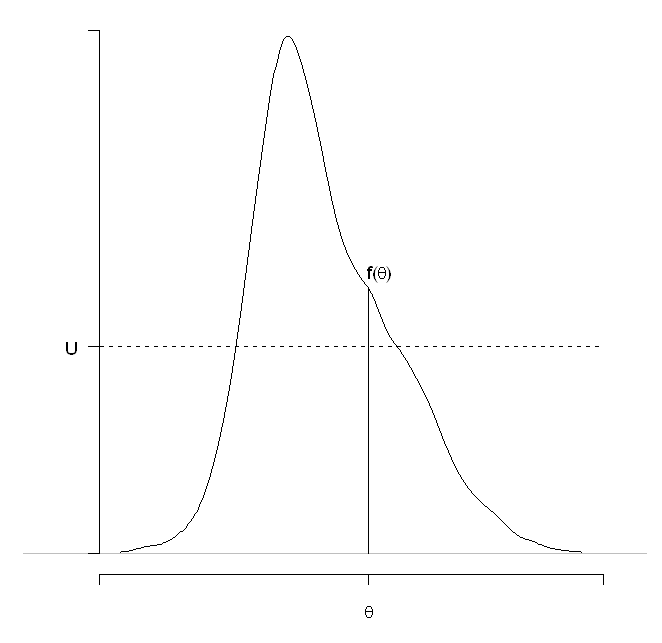
\includegraphics[height=3in]{Ch7/figs/slicesampling}
\end{center}
\caption{Slice sampling. For...}
\label{mcmc.fig.slicesample}
\end{figure}

\footnote{there are supposed to be equations in the caption of figure
4 but it kept causing errors. Rahel: Let me see the equations you want
in there....}

%Slice sampling. For $U \sim Uniform (0, [theta|y])$, we can sample $\theta$ from the vertical slice of $[\theta|y]$ at $U$;  $theta|U \simUnif(B)$, where $B = {theta: U < [theta|y]}$.

Slice sampling can be applied in many situations; however,
implementing an efficient slice sampling procedure can be
complicated. We refer the interested reader to 
\citet[][Chapt. 7]{robert_casella:2010} for a simple example.  Both rejection
sampling and slice sampling can be applied on one-dimensional
conditional distributions within a Gibbs sampling setup.

\section{MCMC for closed capture-recapture Model Mh}
\begin{comment}
\subsection{Building your own MCMC algorithm}
% subsection needed here? maybe not?
\end{comment}

By now you have seen MCMC samplers for some simple GL(M)M's. Now, to
ease you into more complex models, we construct our own MCMC algorithm
using a Metropolis-within-Gibbs sampler for the non-spatial Model with
individual heterogeneity in capture probability $M_{h}$, developed in
Chapt. \ref{chapt.closed}.

To recapitulate: Under the non-spatial model, each of the $n$ observed
individuals is either detected (1) or not (0) during each of $K$
sampling occasions. We estimate $N$ using data augmentation and have a
Bernoulli model for the zero-inflation variables $z_{i}$. 
\[
z_{i} \sim Bernoulli(\psi)
\]
The binomial
observation model is expressed conditional on the latent variables
$z_{i}$. 
\[
y_i \sim Binomial (p_i * z_i, K)
\]
Further, we prescribe a distribution for the capture
probability $p_{i}$. Here we assume
\[
\mathrm{logit}(p_{i}) \sim \mbox{Normal}(\mu,\sigma^2)
\]

As usual, we have to go through two general steps before we write the MCMC algorithm:
\begin{itemize}
\item[  (1)] Identify your model with all its components (including
    priors)
\item[  (2)] Recognize and express the full conditional distributions for
    all parameters
\end{itemize}
Our model components are as follows: $[y_{i}| p_{i},z_{i}]$,
$[p_{i}|\mu_{p},\sigma_{p}]$, and $[z_{i}|\psi]$
for {\it each} $i=1,2,\ldots,M$ and then prior distributions
$[\mu_{p}]$, $[\sigma_{p}]$ and $[\psi]$.
The joint posterior distribution of all unknown quantities in the model
is proportional to the joint distribution of all elements
$y_{i},p_{i},z_{i}$ and also the prior distributions of the prior parameters:
\[
\left\{ \prod_{i=1}^{M} [y_{i}|p_{i},z_{i}][p_{i}|\mu_{p},\sigma_{p}]
[z_{i}|\psi] \right\} [\mu_{p},\sigma_{p},\psi]
\]
For prior distributions, we assume that $\mu_{p},\sigma_{p}, \psi$ are
mutually independent and for $\mu_{p}$ and $\sigma_{p}$ we use
improper uniform priors, and $\psi \sim \mbox{Unif}(0,1)$.  This is equivalent to $\mbox{Beta}(1,1)$, which will come in handy, as we will see in a moment. Note that
the likelihood contribution for each individual, when conditioned on
$p_{i}$ and $z_{i}$, does not depend on $\psi$, $\mu_{p}$, or
$\sigma_{p}$.  As such, the full-conditional for the structural
parameter $\psi$ only depend on the collection of data augmentation
variables $z_{i}$, and that for $\mu_{p}$ and $\sigma_{p}$ will only
depend on the collection of latent variables $p_{i}; i=1,2,\ldots,M$.
The full conditionals for all the unknowns are as follows:

{\bf (1)} For $p_{i}$:
\begin{eqnarray*}
[p_{i}|y_{i}, \mu_p, \sigma_{p},z_{i}=1] &\propto  &
[y_{i}|p_{i}][p_{i}|\mu_p,\sigma_{p}^{2}] \mbox{ if $z_{i}=1$ }  \\
                 &  &  [p_{i}|\mu_p,\sigma_{p}] \mbox{ if $z_{i}=0$ }
\end{eqnarray*}

XXX Andy, is the $z_i = 1$ on the left side supposed to be in there? You have the if $z=1$ and $z=0$ on the right hand side XXXXX
XXX do the parameters that define the prior distribution go into the left side of the equation? Eg for p (above) you have mu and sigma on the left hand side,
so for z should it be [z|y,p,psi]? XXXXX

{\bf (2)} for $z_{i}$:
\[
[z_{i} | y_{i}, p_{i}] \propto [y_{i}|z_{i}*p_{i}] \mbox{Bern}(z_{i}|\psi)
\]

{\bf (3)} For $\mu_{p}$:
\[
[\mu_{p} | p_{i}, \sigma_{p}] \sim \left\{ \prod_{i} [p_{i}|\mu_{p}, \sigma_{p}] \right\} *\mbox{const}
\]


{\bf (4)} For $\sigma_{p}$:
\[
[ \sigma_{p}|p_{i}, \mu_{p} ] \sim \left\{ \prod_{i}[p_{i}| \mu_{p},\sigma_{p} ] \right\} *\mbox{const}
\]

{\bf (5)} For $\psi$:
\[
[\psi|z_{i}] \sim \propto \left\{ \prod_{i} [z_{i}|\psi] \right\} \mbox{Beta}(1,1)
\]
Remember that \mbox{Beta}(1,1) is equivalent to \mbox{Unif}(0,1). The Beta distribution is the conjugate prior to the Binomial and 
Bernoulli distributions and the general form of a full conditional of a Beta-Binomial model 
with $x_{i} \sim \mbox{Bern} (p) $ and $p \sim \mbox{Beta}(a,b)$ is
\[
[p|{\bf x}] \propto \mbox{Beta}(a + \sum_i x_i, b + n-\sum_i x_i)
\]
In our case that means
\[
[\psi|z_{i}] \sim \mbox{Beta}(1 + \sum z_{i}, 1 + M - \sum z_{i})
\]

What we've done here is identify each of the full conditional
distributions in sufficient detail to toss them into our
Metropolis-Hastings algorithm (the constant term in the full conditionals for $\mu_{p}$ and $\sigma_{p}$ reflects the improper prior we chose for both parameters). 
Below, you see the updating step for the detection parameter ${\bf p}$. Note that (1) we draw candidate values on the logit scale and (2) instead of looping through 1 -- M individuals to update all $p_{i}$, we update all elements of the vector of {\bf p} in parallel.   

\begin{verbatim}

### update the logit(p) parameters
lp.cand<- rnorm(M,lp,1)  # 1 is a tuning parameter
p.cand<-plogis(lp.cand)
ll<-dbinom(ytot,K,z*p, log=T)
prior<-dnorm(lp,mu,sigma, log=T)
llcand<-dbinom(ytot,K,z*p.cand, log=T)
prior.cand<-dnorm(lp.cand,mu,sigma, log=T)

kp<- runif(M) < exp((llcand+prior.cand)-(ll+prior))
p[kp]<-p.cand[kp]
lp[kp]<-lp.cand[kp]

\end{verbatim}

Updating the $z_{i}$ is essentially analogous to updating the $p_{i}$ (although they can be updated directly from their full-conditional). $\mu_{p}$ and $\sigma_{p}$ are also updated using MH steps (see the code for $\mu_{p}$ below). In truth, we could also sample $\mu_{p}$
and $\sigma_{p}^{2}$ directly with certain choices of prior
distributions. For example, if $\mu_{p} \sim \mbox{Norm}(0, 1000)$
then the full conditional for $\mu_{p}$ is also normal (see
sec. \ref{mcmc.sec.gibbs}), etc..

\begin{verbatim}

p0.cand<- rnorm(1,p0,.05)
if(p0.cand>0 & p0.cand<1){
mu.cand<-log(p0.cand/(1-p0.cand))
ll<-sum(dnorm(lp,mu,sigma,log=TRUE))
llcand<-sum(dnorm(lp,mu.cand,sigma,log=TRUE))
if(runif(1)<exp(llcand-ll)) {
 mu<-mu.cand
 p0<-p0.cand
}
}

\end{verbatim}

Finally, for $\psi$ we can easily sample directly from the beta distribution:

\begin{verbatim}
psi<-rbeta(1, sum(z) + 1, M-sum(z) + 1)
\end{verbatim}

You can check out the full code by invoking \mbox{\tt modelMh()} from the {\bf R} package \mbox{\tt scrbook}.\footnote{Andy, we could put the analysis of the bear data in here as an exercise.} 

\section{MCMC algorithm for the basic spatial capture-recapture model}

Conceptually, but also in terms of MCMC coding, it is only a small step from the non-spatial model Mh to a fully spatial capture-recapture model. Next, we'll walk you through the steps of building your own MCMC sampler for the basic SCR model (i.e. without any individual, site or time specific covariates) with both a Poisson and a Binomial encounter process.
As usual, we will have to go through two general steps before we write the MCMC algorithm:
\begin{itemize}
\item[  (1)] Identify your model with all its components (including
    priors)
\item[  (2)] Recognize and express the full conditional distributions for
    all parameters
\end{itemize}
It is worthwhile to go through all of step 1 for an SCR model, but you
have probably seen enough of step 2 in our previous examples to get
the essence of how to express a full conditional
distribution. Therefore, we will exemplify step 2 for some parameters
and tie these examples directly to the respective R code.

{\bf Step 1 -- Identify your model}

Recall the components of the basic SCR model with a Poisson encounter process from Chapt. \ref{chapt.poisson-mn}:
We assume that individuals $i$, or rather, their activity centers
${\bf s}_i$, are uniformly distributed across the state space ${\cal S}$,
\[
{\bf s}_i  \sim \mbox{Unif}({\cal S})
\]
and that the number of times individual $i$ encounters trap $j$, $y_{ij}$, is a random Poisson variable with mean $\lambda_{ij}$,
\[
y_{ij} \sim \mbox{Poisson}(\lambda_{ij})
\]
The link between individual location, movement and trap encounter
rates is made by the assumption that $\lambda_{ij}$, is a decreasing
function of the distance between ${\bf s}_i$ and the location of $j$,
${\bf x}_{j}$, say $D_{ij} = ||{\bf s}_{i} - {\bf x}_{j}||$, of the half-normal form
\[
\lambda_{ij} =  \lambda_0  \exp(-D_{ij}^2/2\sigma^2),
\]
where $\lambda_0$ is the baseline trap encounter rate at $D_{ij}=0$ and $\sigma$ controls the shape of the half-normal function.

In order to estimate the number of ${\bf s}_i$ in ${\cal S}$ (or any
subset of ${\cal S}$), $N$, we use data augmentation (sec. \ref{closed.sec.da}) and create $M-n$ all-0 encounter histories, where $n$ is the number of individuals we observed and $M$ is a somewhat arbitrary number that is larger than $N$. We estimate $N$ by summing over the auxiliary data augmentation variables, $z_i$, which is 1 if the individual is part of the population and 0 if not, and assume that $z_i$ is a random Bernoulli variable,
\[
z_{i} \sim \mbox{Bern}(\psi)
\]

To link the two model components, we modify our trap encounter model to
\[
\lambda_{ij} = \lambda_0 * exp(-D_{ij}^2/2\sigma^2) * z_{i}.
\]
The model has the following structural parameters, for which we need to specify priors:
\begin{itemize}
\item[ $\psi$:] the $\mbox{Unif}(0,1)$ is required as part of the data augmentation procedure and in general is a natural choice of an uninformative prior for a probability. It will also lead to conjugacy as we saw in the example of model Mh, so that we can update $\psi$ directly from its full conditional distribution using Gibbs sampling.
\item[ ${\bf s}_{i}$:] since ${\bf s}_{i}$ is a pair of coordinates it is two-dimensional and we use a uniform prior limited by the extent of our state-space over both dimensions.
\item[ $\sigma$:] we can conceive several priors for $\sigma$ but let's assume an improper prior, one that is Uniform over $(-\infty, \infty)$. We will see why this is convenient when we construct the full conditionals for $\sigma$.
\item[ $\lambda_{0}$:] analogous, we will use a $\mbox{Unif}(-\infty, \infty)$ improper prior for $\lambda_{0}$.
\end{itemize}
The parameter that is the objective of our modeling, $N$, is a derived parameter that we can simply obtain by summing all $z_i$:
\[
N = \sum_{i=1}^{M} z_{i}
\]

{\bf Step 2 -- Construct the full conditionals:}
Having completed step 1, let's look at the full conditional distributions for some of these parameters.
We find that with improper priors, full conditionals are proportional only to the likelihood of the observations; for example, take the movement parameter $\sigma$:
\[
[\sigma|{\bf s}, \lambda_{0}, {\bf z}, {\bf y}] \propto \left\{ \prod_{i} [y_{i}| {\bf
    s}_{i}, \lambda_{0}, z_{i}, \sigma] \right\} * [\sigma]
\]
Since the improper prior implies that $[\sigma] \propto 1$, we can reduce this further to
\[
[\sigma|{\bf s}, \lambda_{0}, {\bf z}, {\bf y}] \propto \left\{
  \prod_{i} [y_{i}| {\bf s}_{i}, \lambda_{0}, z_{i}, \sigma] \right\}
\]
The {\bf R} code to update $\sigma$ is shown below.
Notice that we automatically reject negative candidate values, since $\sigma$ cannot be $<0$.  

\begin{verbatim}
sig.cand <- rnorm(1, sigma, 0.1)	#draw candidate value
 if(sig.cand>0){   #automatically reject sig.cand that are <0
     lam.cand <- lam0*exp(-(D*D)/(2*sig.cand*sig.cand))
     ll<- sum(dpois(y, lam*z, log=TRUE))
     llcand <- sum(dpois(y, lam.cand*z, log=TRUE))
     if(runif(1) < exp( llcand  - ll) ){
         ll<-llcand
         lam<-lam.cand
         sigma<-sig.cand
      }
  }
\end{verbatim}

These steps are analogous for  $\lambda_{0}$ and ${\bf s}_i$ and we will 
use MH steps for
all of these parameters. Similar to the random intercepts in our
Poisson GLMM, we update each ${\bf s}_i$ individually. Note that to be fully
correct, the full conditional for ${\bf s}_i$ contains both the likelihood and
prior component, since we did not specify an improper, but a Uniform
prior on ${\bf s}_i$. However, with a Uniform distribution the probability
density of any value is 1/(upper limit - lower limit) =
constant. Thus, the prior components are identical for both the
current and the candidate value and can be ignored (formally, when you
calculate the ratio of posterior densities, $r$, the identical prior
component appears both in the numerator and denominator, so that they
cancel each other out).

We still have to update $z_i$. The full conditional for $z_i$ is
\[
[z_i|y_{i}, \sigma, \lambda_0, {\bf s}_{i}] \propto [y_{i}|z_{i},\sigma, \lambda_0, 
{\bf s}_{i}] * [z_i]
\]
and since $z_i \sim Bernoulli(\psi)$,
the term has to be taken into account when updating $z_i$:

\begin{verbatim}
        zUps <- 0		#set counter to monitor acceptance rate
        for(i in 1:M) {
            if(seen[i])	#no need to update seen individuals, since their z =1
                next
            zcand <- ifelse(z[i]==0, 1, 0)
            llz <- sum(dpois(y[i,],lam[i,]*z[i], log=TRUE))
            llcand <- sum(dpois(y[i,], lam[i,]*zcand, log=TRUE))

            prior <- dbinom(z[i], 1, psi, log=TRUE)
            prior.cand <- dbinom(zcand, 1, psi, log=TRUE)
            if(runif(1) < exp( (llcand+prior.cand) - (llz+prior) )) {
                z[i] <- zcand
                zUps <- zUps+1
            }
        }
\end{verbatim}

$\psi$
 is a hyperparameter of the model, with an uninformative prior 
 distribution of $\mbox{Unif}(0,1)$ or $\mbox{Beta}(1,1)$, so that
\[
[psi|{\bf z}] \propto \mbox{Beta}(1 + \sum_i z_i, 1 + M-\sum_i z_i)
\]


These are all the building blocks you need to write the MCMC algorithm
for the spatial null model with a Poisson encounter process.  You can
find the full {\bf R} code by calling the function (\mbox{\tt SCR0pois()}) in the {\bf R} package 
\mbox{\tt scrbook}.

\subsection{SCR model with binomial encounter process}
The equivalent SCR model with a binomial encounter process is very similar. Here, each individual $i$ can only be detected once at any given trap $j$ during a sampling occasion $k$.
Thus
\[
y_{ij} \sim \mbox{Bin} (p_{ij}, K)
\]
Where $p_{ij}$ is some function of distance between ${\bf s}_{i}$ and trap location ${\bf x}_{j}$. Here we use:
\[
p_{ij}=1-exp(-\lambda_{ij})
\]
Recall from Chapt. \ref{chapt.glms} that this is the complementary log-log (cloglog) link function, which constrains $p_{ij}$ 
to fall between 0 and 1.
For our MCMC algorithm that means that, instead of using a Poisson 
likelihood, $\mbox{Poisson}(y|\sigma,\lambda_0,{\bf s},z)$, we use a 
Binomial likelihood, $\mbox{Bin}(y| \sigma,\lambda_0,{\bf s},z; K)$, 
in all the conditional distributions. An exemplary updating step for $\lambda_0$ under a Binomial encounter model is shown below. 
The full MCMC code for the Binomial SCR with a clog-log link (\mbox{\tt SCR0binom.cl()}) 
can be found in the {\bf R} package \mbox{\tt scrbook}.

\begin{verbatim}

        lam0.cand <- rnorm(1, lam0, 0.1)
        if(lam0.cand >0){   #automatically reject lam0.cand that are <0
            lam.cand <- lam0.cand*exp(-(D*D)/(2*sigma*sigma))
            p.cand <- 1-exp(-lam.cand)
            ll<- sum(dbinom(y, K, pmat *z, log=TRUE))  
            llcand <- sum(dbinom(y, K, p.cand *z, log=TRUE))
            if(runif(1) < exp( llcand  - ll) ){
                ll<-llcand
                pmat<-p.cand
                lam0<- lam0.cand
            }
        }
\end{verbatim}

Another possibility is to model variation in the individual and site 
specific detection probability,  $p_{ij}$, directly, without any 
transformation, such that
\begin{comment} Rahel the $\leftarrow$ isn't right here but I couldn't
make this work 
What's wrong with a '=' ?
\end{comment}
\[
p_{ij} = p_0 * exp(-D_{ij}^2/(2\sigma^2))
\]
and $p_0 \in [0,1]$.
This formulation is analogous to how detection probability is modeled 
in distance sampling under a half-normal detection function; however, 
in distance sampling $p_0$ -- detection of an individual on the transect 
line -- is assumed to be 1 \citep{buckland_etal:2001}. Under this 
formulation the updater for $p_0$ becomes:

\begin{verbatim}
  p0.cand <- rnorm(1, p0, 0.1)
  if(p0.cand >0 & p0.cand < 1 ){   
      #automatically rejects lam0.cand that are not {0,1}
       p.cand <- p0.cand*exp(-(D*D)/(2*sigma*sigma))
       ll<- sum(dbinom(y, K, pmat *z, log=TRUE)) #no transformation needed
       llcand <- sum(dbinom(y, K, p.cand *z, log=TRUE))
       if(runif(1) < exp( llcand  - ll) ){
          ll<-llcand
            pmat<-p.cand
            p0<- p0.cand
         }
     }
\end{verbatim}


\subsection{Looking at model output}
Now that you have an MCMC algorithm to analyze spatial capture-recapture 
data with, let's run an actual analysis so we can look at the output. As 
an example, we will use the Fort Drum 
bear data set we first introduced in Chapt. \ref{chapt.intro} and already analyzed in Chapt. \ref{chapt.closed} with 
traditional non-spatial models (and that you will see again in Chapt. 
\ref{chapt.covariates}). You can load the Fort Drum data
(\mbox{\tt data(beardata) }), extract the 
trap locations (\mbox{\tt trapmat}) and 
detection data (\mbox{\tt bearArray}) and build the augmented $M \times J$ array of individual 
encounter histories:
\begin{verbatim}
M=700
bearmat<-apply(bearArray, 1:2, sum) #summarizes captures across occasions
Xaug<-matrix(0, nrow=M, ncol=dim(trapmat)[1])
Xaug[1:dim(bearmat)[1],]<-bearmat  #create augmented data set
\end{verbatim}

 In addition to these data, we need to specify 
the outermost coordinates of the state-space. Since bears are wide 
ranging animals we add a 20--km buffer to the maximum and minimum 
coordinates of the trap array:

\begin{verbatim}
xl<- min(trapmat[,1])- 20  
yl<- min(trapmat[,2])- 20 
xu<- max(trapmat[,1])+ 20
yu<- max(trapmat[,2])+ 20
\end{verbatim}

Finally, use the MCMC code for the binomial encounter model
with the clog-log link  ({\tt SCR0binom.cl}) and run 5000 iterations. This should take 
approximately 25 minutes (in real life we would of course run the algorithm a lot longer but for demonstration purposes let's stick with a number of iterations that can be run in a manageable amount of time).
%need to look at tuning... not happy
\begin{verbatim}
set.seed(13)
 mod0<-SCR0binom.cl(y=Xaug, X=trapmat, M=M, xl=xl, xu=xu, yl=yl, 
                   yu=yu, K=8, delta=c(0.1, 0.05, 2), niter=5000)
\end{verbatim}

Before, we used simple {\bf R} commands to look at model results. 
However, there is a specific {\bf R} package to summarize MCMC 
simulation output and perform some convergence diagnostics -- package 
coda \citep{plummer_etal:2006}. Download and install coda, then 
convert your model output to an mcmc object
\begin{verbatim}
  chain<-mcmc(mod0)
\end{verbatim} 
which can be used by coda to produce MCMC specific output.

\subsubsection{Markov chain time series plots}

Start by looking at time series plots of your Markov chains using 
\verb#plot(chain)#. This command produces a time series plot and
 marginal posterior density plots for each monitored parameter, 
 similar to what we did before using the \verb#hist()# and \verb#plot()# 
 commands. Fig. \ref{mcmc.fig.timeseries} shows an example of these plots for $\sigma$ and $\lambda_0$. Time series plots will tell 
 you several things:
First, recall from Sect. \ref{Metropolis-Hastings sampling} that the way the chains move 
through the parameter space gives you an idea of whether your MH 
steps are well tuned. If chains were constant over many iterations 
you would need to decrease the tuning parameter of the (Normal) 
proposal distribution. If a chain moves along some gradient to a 
stationary state very slowly, you may want to increase the tuning 
parameter so that the parameter space is explored more efficiently.


\begin{figure}
\begin{center}
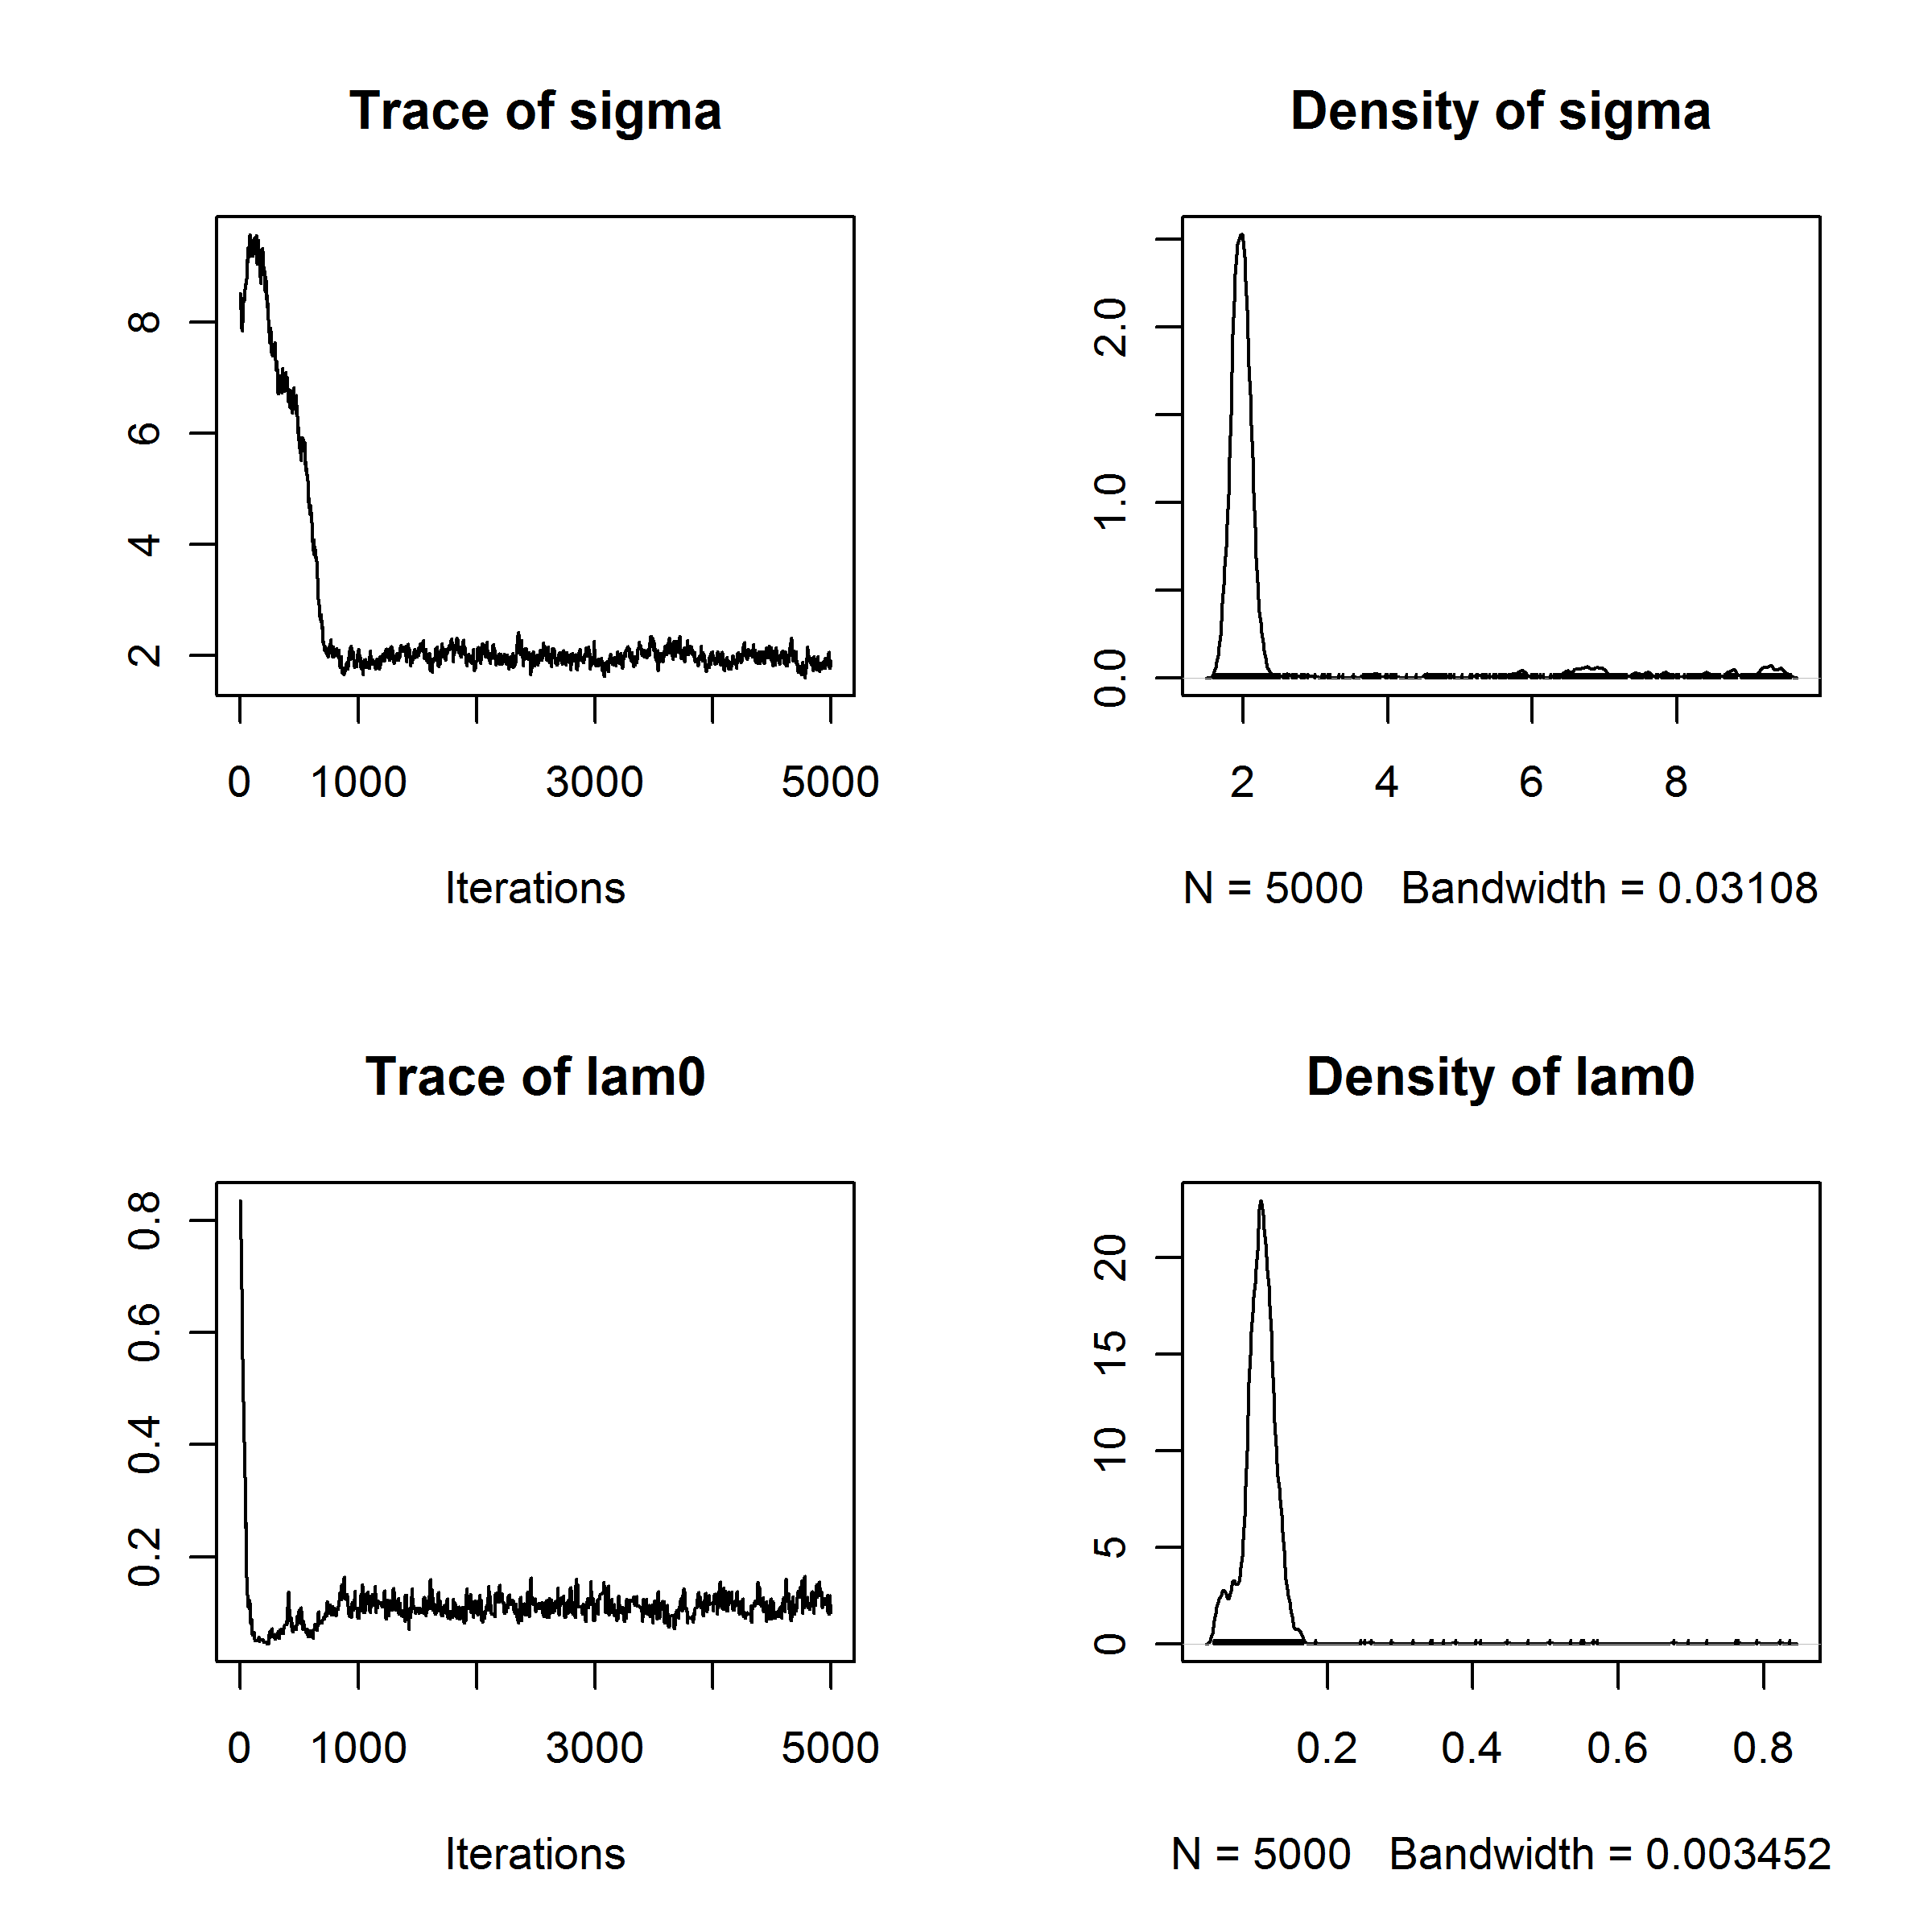
\includegraphics[height=2.5in]{Ch7/figs/timeseries}
\end{center}
\caption{Time series and posterior density plots for $\sigma$ and $\lambda_0$.}
\label{mcmc.fig.timeseries}
\end{figure}


Second, you will be able to see if your chains converged and how many initial simulations you have to discard as burn-in. In the case of the chains shown in Fig. \ref{mcmc.fig.timeseries}, we would probably consider the first 750 -- 1000 iterations as burn-in, as afterwards the chains seem to be fairly stationary.

\subsection{Posterior density plots}
The \verb#plot()# command also produces posterior density plots and it is worthwhile to look at those carefully. For parameters with priors that have bounds (e.g. Uniform over some interval), you will be able to see if your choice of the prior is truncating the posterior distribution. In the context of SCR models, this will mostly involve our choice of $M$, the size of the augmented data set. If the posterior of $N$ has a lot of mass concentrated close to $M$ (or equivalently the posterior of $\psi$ has a lot of mass concentrated close to 1), as in the example in Fig. \ref{timeseries2.fig}, we have to re-run the analysis with a larger $M$.  A diffuse
posterior plot suggests
that the parameter may not be well-identified. 
There may not be enough information in your data to estimate model parameters and you may have to consider a simpler model. Finally, posterior density plots will show you if the posterior distribution is symmetrical or skewed -- if the distribution has a heavy tail, using the mean as a point estimate of your parameter of interest may be biased and you may want to opt for the median or mode instead.

\begin{figure}
\begin{center}
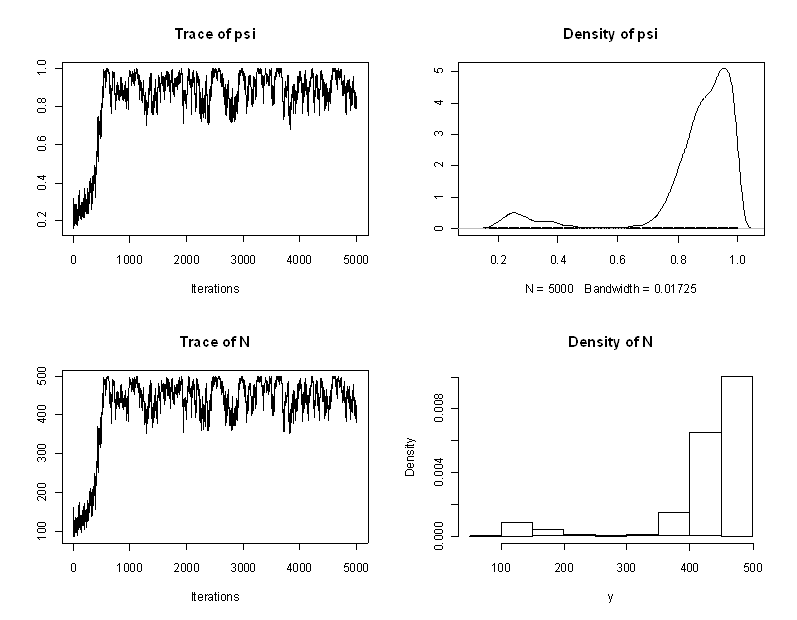
\includegraphics[height=2.5in]{Ch7/figs/timeseries2}
\end{center}
\caption{Time series and posterior density plots of $\psi$ and $N$ for the bear data set truncated by the upper limit of $M$ (500).}
\label{timeseries2.fig}
\end{figure}

\subsection{Serial autocorrelation and effective sample size}

Checking the degree of autocorrelation in your Markov chains and 
estimating the effective sample size your chain has generated should 
be part of evaluating your model output. If you use {\bf WinBUGS}
 through the \mbox{\tt R2WinBUGS} package, the \verb#print()# command 
 will automatically return the effective sample size for all monitored 
 parameters. In the coda package there are several functions you can use 
 to do so. \verb#effectiveSize()# will directly give you an estimate 
 of the effective sample size for you parameters:
\begin{verbatim}
> effectiveSize(chain)
    sigma      lam0       psi         N
 3.930303 78.259159 30.436348 32.047392
\end{verbatim}

Alternatively, you can use the \verb#autocorr.diag()# function, which will show you the degree of autocorrelation for different lag values (which you can specify within the function call, we use the defaults below):
\begin{verbatim}
> autocorr.diag(mcmc(mod))
           sigma      lam0       psi         N
Lag 0  1.0000000 1.0000000 1.0000000 1.0000000
Lag 1  0.9979948 0.9494134 0.9847503 0.9774201
Lag 5  0.9915567 0.8038168 0.9111951 0.9113525
Lag 10 0.9836016 0.6714021 0.8462108 0.8509803
Lag 50 0.8985337 0.1983780 0.6138516 0.6233994
\end{verbatim}
In the present case we see that autocorrelation is especially high for the 
parameter $\sigma$ and our effective sample size for this parameter is 
4! \footnote{Anyone have any idea how the autocorrelation in sigma could 
be reduced? XXXXXXXXXX YES: Mess with the MH tuning parameter......XXXXXXXX} 
This means we would have to run the model for much longer to 
obtain a reasonable effective sample size. Unfortunately, with many SCR models we observe high degrees of serial autocorrelation. For now, let's continue using this small set of samples to continue looking at the output.


\subsection{Summary results}
\label{mcmc.sec.mcmcsummary}

Now that we checked that our chains apparently have converged and pretending 
that we have generated enough samples from the posterior distribution, we 
can look at the actual parameter estimates. The \verb#summary()# function 
will return two sets of results: the mean parameter estimates, with their standard deviation, the na\'{i}ve standard error -- i.e. your regular standard error calculated for $T$ (= number of iterations) 
samples without 
accounting for serial autocorrelation -- and the 
Time-series SE (in {\bf WinBUGS} 
and earlier in this book referred to as MC error), which accounts for 
autocorrelation. Remember our rule of thumb that this error 
decreases with increasing chain length and should be 1\% or less of the 
parameter estimate. In {\bf WinBUGS} the MC error is only given in the log 
output within {\bf BUGS} itself.
You should adjust the \verb#summary()# call by removing the burn-in from
calculating parameter summary statistics. To do so, use the \verb#window()#
command, which lets you specify at which iteration to start
'counting'. In contrast to {\bf WinBUGS}, which requires you to set the
burn-in length before you run the model, this command gives us full
flexibility to make decisions about the burn-in after we have seen the
trajectories of our Markov chains. For our example,
\verb#summary(window(chain, start=1001))# returns the following output:


\begin{verbatim}
Iterations = 1001:5000
Thinning interval = 1
Number of chains = 1
Sample size per chain = 4000

1. Empirical mean and standard deviation for each variable,
   plus standard error of the mean:

          Mean       SD  Naive SE Time-series SE
sigma   1.9986  0.13805 0.0021827       0.016091
lam0    0.1096  0.01523 0.0002407       0.001401
psi     0.6113  0.09148 0.0014465       0.010734
N     489.8535 71.79695 1.1352094       8.431119

2. Quantiles for each variable:

           2.5%       25%      50%      75%    97.5%
sigma   1.75780   1.89847   1.9900   2.0944   2.2772
lam0    0.08357   0.09824   0.1087   0.1192   0.1427
psi     0.45110   0.54838   0.6052   0.6639   0.8192
N     366.00000 440.00000 485.0000 530.0000 654.0000
\end{verbatim}

Looking at the MC errors (column labeled \mbox{\tt Time-series SE}), 
we see that in spite of the high autocorrelation, the MC error for 
$\sigma$ is below the 1\% threshold, whereas for all other parameters, 
MC errors are still above, another indication that for a thorough 
analysis we should run a longer chain.

Our algorithm gives us a posterior distribution of $N$, but we are usually 
interested in the density, $D$. Density itself is not a parameter of our 
model, but we can derive a posterior distribution for $D$ by dividing 
each value of $N$ ($N$ at each iteration) by the area of the state-space
 (here 3032.719 km$^2$) and we can use summary statistics of the 
 resulting distribution to characterize $D$:
\begin{verbatim}
> summary(window(chain[,4]/ 3032.719, start=1001))
Iterations = 1001:5000
Thinning interval = 1
Number of chains = 1
Sample size per chain = 4000

1. Empirical mean and standard deviation for each variable,
   plus standard error of the mean:

          Mean             SD       Naive SE Time-series SE
     0.1615229      0.0236741      0.0003743      0.0027801

2. Quantiles for each variable:

  2.5%    25%    50%    75%  97.5%
0.1207 0.1451 0.1599 0.1748 0.2156
\end{verbatim}
We see that our mean density of $0.16/km^2$ is very similar to the estimate of $0.18/km^2$ obtained under the non-spatial model M0 in Chapt. \ref{chapt.closed}.


\subsection{Other useful commands }
While inspecting the time series plot gives you a first idea of how well you tuned your MH algorithm, use \verb#rejectionRate()# to obtain the rejection rates (1 -- acceptance rates) of the parameters that are written to your output:
\begin{verbatim}
> rejectionRate(chain)
     sigma       lam0        psi          N
0.44108822 0.77675535 0.00000000 0.01940388
\end{verbatim}
 Recall (\ref{Metropolis-Hastings sampling}) that rejection rates should lie between 0.2 and 0.8, so our tuning seems to have been appropriate here. $\psi$ is never rejected since we update it with Gibbs sampling, where all candidate values are kept. And since $N$ is the sum of all $z_i$, all it takes for $N$ to change from one iteration to the next are small changes in the z-vector, so the rejection rate of $N$ is always low.
If you have run several parallel chains, you can combine them into a single mcmc object using the \verb#mcmc.list()# command on the individual chains (note that each chain has to be converted to an mcmc object before combining them with \verb#mcmc.list()#). You can then easily obtain the Gelman-Rubin diagnostic \citep{gelman_etal:2004}, in {\bf WinBUGS} called R-hat, using \verb#gelman.diag()#, which 
will indicate if all chains have converged to the same stationary distribution.
For details on these and other functions, see the \mbox{\tt coda} manual, 
which can be found (together with the package) on the CRAN mirror.
%%maybe add in Geweke statistic here...

\section{Manipulating the state-space}
\label{mcmc.sec.state-space}

So far, we have constrained the location of the activity centers to fall
within the outermost coordinates of our rectangular state space by posing 
upper and lower bounds for $x$ and $y$. But what if ${\cal S}$ 
has an irregular 
shape -- maybe there is a large water body we would like to remove from 
${\cal S}$, because we know our terrestrial study species does not occur there.
Or the study takes place in a clearly defined area such as an island. 
As mentioned before, this situation is difficult to handle in {\bf WinBUGS}.
In some simple cases we can adjust the state space by setting one of the
coordinates of ${\bf s}_{i}$ to be some function of the other. 
In this manner, we can cut off corners of the rectangle to approximate 
the actual state space. In {\bf R}, we are much more flexible, as we can 
use the actual state-space polygon to constrain out ${\bf s}_i$. 
\footnote{ Have to check if we can use panther stuff for the book; 
otherwise, use raccoon example.} To illustrate that, let's look at a camera 
trapping study of Florida panthers (\emph{Puma concolor coryi}) conducted 
in the Picayune Strand Restoration Project (PSRP) area, southwest Florida 
(Fig. \ref{mcmc.fig.pantercamera}), by XXX, and financed by XXX. In the 1960ies 
the PSRP area was slated for housing development, but then bought back by 
the State of Florida and is currently being restored to its original 
hydrology and vegetation. In an effort to estimate the density of the 
local Florida panther population, 98 camera traps were operated in the area 
for 21 months between 2005 and 2007. Florida panthers are wide-ranging 
animals and in order to account for their wide movements, the state-space 
was defined as the trapping grid buffered by 15 km around its outermost 
coordinates. However, the resulting rectangle contained some ocean in its 
southwestern corner (Fig. \ref{pantercamera.fig}).
In order to precisely describe the state-space, the ocean has to be 
removed. You can create a precise state-space polygon in {\bf ArcGIS} and 
read it into {\bf R}, or create the polygon directly within {\bf R}. In 
the present case we intersected two shape files -- one of the state of 
Florida and one of the rectangle defined by a strip of 15 km around the
 camera-trapping grid.
While you will most likely have to obtain the shapefile describing the 
landscape of and around your trapping grid (coastlines, water bodies etc.) 
from some external source, a polygon shapefile buffering your outermost 
trapping grid coordinates can easily be written in {\bf R}.

If \mbox{\tt xmin}, \mbox{\tt xmax}, \mbox{\tt ymin} and 
\mbox{\tt ymax} mark the most extreme
$x$ and $y$ coordinates of your 
trapping grid and $b$ is the distance you want to buffer with, load the 
package \mbox{\tt shapefiles} \citep{stabler:2006} and issue the following
{\bf R} commands:
\begin{verbatim}
xl= xmin-b
xu= xmax+b
yl= ymin-b
yu= ymax+b

            #create data frame with coordinate pairs
dd <- data.frame(Id=c(1,1,1,1,1),X=c(xl,xu,xu,xl,xl), Y=c(yl,yl,yu,yu,yl)) 
ddTable <- data.frame(Id=c(1),Name=c("Item1"))
            #convert to shapefile, type polygon
ddShapefile <- convert.to.shapefile(dd, ddTable, "Id", 5) 
            # save to location of choice
write.shapefile(ddShapefile, 'c:/Test', arcgis=T) 
\end{verbatim}


\begin{figure}
\begin{center}
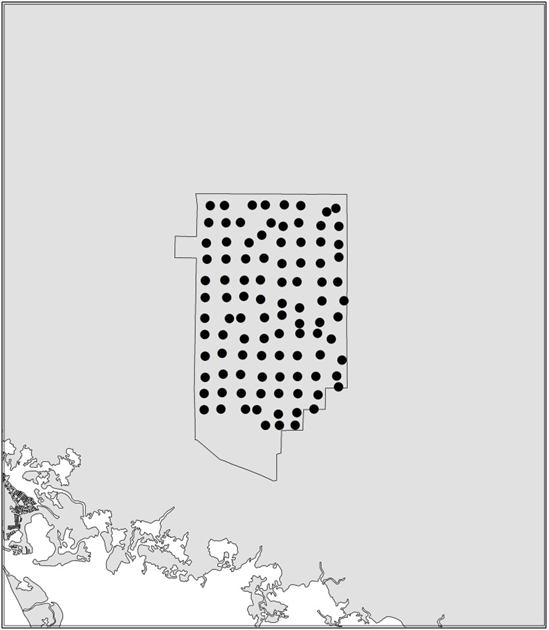
\includegraphics[height=2.5in]{Ch7/figs/panthercamera}
\end{center}
\caption{Rectangular state-space for a Florida panther camera trapping
study in the PSRP area (grey outline, red block inset map of Florida)
contain some ocean (white) that needs to be removed from the state-space.}
\label{mcmc.fig.pantercamera}
\end{figure}

You can read shapefiles into {\bf R} loading the package \mbox{\tt 
maptools}
\citep{lewin-koh_etal:2011} and using the function
\verb#readShapeSpatial()#. Make sure you read in shapefiles in UTM format, so
that units of the trap array, the movement parameter $\sigma$ and the
state-space are all identical.  Intersection of polygons can be done
in {\bf R} also, using the package \mbox{\tt rgeos} 
\citep{bivand_rundel:2011} and the
function \verb#gIntersect()#. The area of your (single) polygon can be
extracted directly from the state-space object \mbox{\tt SSp}:

\begin{verbatim}
 area <- SSp@polygons[[1]]@Polygons[[1]]@area /1000000
\end{verbatim}

 Note that dividing by 1000000 will return the area in km$^2$ if your coordinates describing the polygon are in UTM. If your state-space consists of several disjunct polygons, you will have to sum the areas of all polygons to obtain the size of the state-space.
To include this polygon into our MCMC sampler we need one last spatial 
{\bf R} package, \mbox{\tt sp} \citep{pebesma_bivand:2011}, which has a 
function, \verb#over()#, which allows us to check if a pair of coordinates 
falls within a polygon or not. All we have to do is embed this new check 
into the updating steps for ${\bf s}$:
\begin{verbatim}
    #draw candidate value
Scand <- as.matrix(cbind(rnorm(M, S[,1], 2), rnorm(M, S[,2], 2)))
     #convert to spatial points on UTM (m) scale
Scoord<-SpatialPoints(Scand*1000)   
     # check if scand is within the polygon
SinPoly<-over(Scoord,SSp)		

for(i in 1:M) {
    #if scand falls within polygon, continue update
   if(is.na(SinPoly[i])==FALSE) {		
... [rest of the updating step remains the same]
\end{verbatim}
Note that it is much more time-efficient to draw all $M$ candidate values 
for $s$ and check once if they fall within the state-space, rather than 
running the \verb#over()# command for every individual pair of 
coordinates. To make sure that our initial values for {\bf s} also fall 
within the polygon of ${\cal S}$, we use the function \verb#runifpoint()# 
from the package \mbox{\tt spatstat} \citep{baddeley_turner:2005}, 
which generates random uniform points within a specified polygon. You'll 
find this modified MCMC algorithm (\mbox{\tt SCR0poisSSp()}) in the {\bf R} 
package \mbox{\tt scrbook}.
%need to add and check this piece of code
Finally, observe that we are converting candidate coordinates of ${\cal S}$ 
back to meters to match the UTM polygon. In all previous examples, 
for both the trap locations and the activity centers we have used UTM 
coordinates divided by 1000 to estimate $\sigma$ on a km scale. This is 
adequate for wide ranging species like bears. In other cases you 
may center all coordinates on 0. No matter what kind of transformation you 
use on your coordinates , make sure to always convert candidate values for 
${\cal S}$ back to the original scale (UTM) before running the 
\verb#over()# command.

\section{MCMC software packages}

Throughout most of this book we will use {\bf WinBUGS} and, occasionally, {\bf JAGS} to run MCMC analyses. 
Here, we will briefly discuss the main pros and cons of these two programs 
as well as {\bf WinBUGS} successor {\bf OpenBUGS}. 

\subsection{WinBUGS}

In a nutshell, {\bf WinBUGS} (and the other programs) do everything that we 
just went through in this chapter (and quite a bit more). Looking through 
your model, {\bf WinBUGS} determines which parameters it can use standard 
Gibbs sampling for (i.e. for conjugate full conditional distributions). 
Then, it determines, in the following hierarchy, whether to use adaptive 
rejection sampling, slice sampling or -- in the `worst' case -- 
Metropolis-Hastings sampling for the other full conditionals 
\citep{spiegelhalter_etal:2003}. If it uses MH sampling, it will 
automatically tune the updater so that it works efficiently.
While {\bf WinBUGS} is a convenient piece of software that is still 
widely used, its major drawback is that it is no longer being developed, 
i.e. no new functions or distributions are added and no bugs are fixed.

\subsection{OpenBUGS}
{\bf OpenBUGS} is essentially the successor of {\bf WinBUGS}. While the 
latter is
no longer actively developed, {\bf OpenBUGS} continues to be 
developed. The
name '{\bf OpenBUGS}' refers to the software being open source, so users 
do
not need to download a license key, like they have to for {\bf WinBUGS}
(although the license key for {\bf WinBUGS} is free and valid for life).

Compared to {\bf WinBUGS}, {\bf OpenBUGS} 
has  more built-in functions. The
method of how to determine the right updater for each model parameter
has changed and the user can manually control the MCMC algorithm used
to update model parameters.  Several other changes have been
implemented in {\bf OpenBUGS} and a detailed list of differences between the
two {\bf BUGS} versions, can be found at
\url{http://www.openbugs.info/w/OpenVsWin}.

While {\bf OpenBUGS} is a useful program for a lot of MCMC sampling
applications, for reasons we do not understand, simple SCR models do
not converge sometimes in {\bf OpenBUGS}. It is therefore advisable that 
you check any
{\bf OpenBUGS} SCR model results against result from {\bf WinBUGS}. Also,
currently, the {\bf R} package \mbox{\tt BRugs} \citep{thomas_etal:2006}, 
necessary
for running {\bf OpenBUGS} through {\bf R}, has problems with 64-bit 
machines, so
you may have to use the 32-bit version of {\bf R} and {\bf OpenBUGS} 
in order to
make it work. The {\bf BUGS} project site at 
\url{http://www.openbugs.info}
provides a lot of information on and download links for {\bf OpenBUGS}.

There is an extensive help archive for both {\bf WinBUGS} and {\bf OpenBUGS}
 and you can subscribe to a mailing list, where people pose and answer 
 questions of how to use these programs at 
 \url{http://www.mrc-bsu.cam.ac.uk/bugs/overview/list.shtml}

\subsection{JAGS -- Just Another Gibbs Sampler}

{\bf JAGS}, currently at Version 3.1.0, is another free program for analysis 
of Bayesian hierarchical models using MCMC simulation. Originally, {\bf JAGS}
 was the only program using the {\bf BUGS} language that would run on 
 operating systems other than the 32 bit Windows platforms. By now, there 
 are {\bf OpenBUGS} versions for Linux or Macintosh machines.
{\bf JAGS} 'only' generates samples from the posterior distribution; 
analysis of the output is done in {\bf R}, either by running {\bf JAGS} 
through {\bf R} using either the packages \mbox{\tt rjags} 
\citep{plummer:2011} or \mbox{\tt R2jags} \citep{su_yajima:2011}, or by 
using coda on your {\bf JAGS} output. The program, manuals and \mbox{\tt rjags} 
can be downloaded at \url{http://sourceforge.net/projects/mcmc-jags/files/}
When run from within {\bf R} using the package \mbox{\tt rjags} or \mbox{R2jags}, 
writing a \mbox{\bf JAGS} model is virtually identical to writing a {\bf WinBUGS}
 model. However, some functions may have slightly different names and you 
 can look up available functions and their use in the {\bf JAGS} 
 manual. One potential downside is that {\bf JAGS} can be very particular 
 when it comes to initial values. These may have to be set as close to 
 truth as possible for the model to start. Although {\bf JAGS} lets 
 you run several parallel Markov chains, this characteristic interferes 
 with the idea of using overdispersed initial values for the different 
 chains. Also, we have occasionally experienced {\bf JAGS} to crash and 
 take the {\bf R} GUI with it. Only re-installing both {\bf JAGS} and 
 {\tt rjags} seemed to solve this problem.
On the plus side, {\bf JAGS} usually runs a little faster than {\bf WinBUGS},
 sometimes considerably faster (see Sect. \ref {4.XYZ}), is constantly 
 being developed and improved and it has a variety of functions that are 
 not available in {\bf WinBUGS}. For example, {\bf JAGS} allows you to 
 supply observed data for some deterministic functions of unobserved 
 variables. In {\bf BUGS} we cannot supply data to logical nodes. 
 Another useful feature is that the adaptive phase of the model 
 (the burn-in) is run separately from the sampling from the stationary 
 Markov chains. This allows you to easily add more iterations to the 
 adaptive phase if necessary without the need to start from 0. There 
 are other, more subtle differences and there is an entire manual section 
 on differences between {\bf JAGS} and {\bf OpenBUGS}.
For questions and problems there is a {\bf JAGS} forum online at 
\url{http://sourceforge.net/projects/mcmc-jags/forums/forum/610037}.
\footnote{As we make progress on the book, lets be sure  to add 
linkages to places where we use JAGS in examples.}

\section{Summary and Outlook}

Although there are a number of flexible and extremely useful software 
packages to perform MCMC simulations, it sometimes is more efficient to 
develop your own MCMC algorithm. Building an MCMC code follows three basic 
steps: Identify your model including priors and express full conditional 
distributions for each model parameter. If full conditionals are parametric 
distributions, use Gibbs sampling to draw candidate parameter values from 
those distributions; otherwise use Metropolis-Hastings sampling to draw 
candidate values from a proposal distribution and accept or reject them 
based on their posterior probability densities.
These custom-made MCMC algorithms give you more modeling flexibility than 
existing software packages, especially when it comes to handling the
 state-space: In {\bf BUGS} (and {\bf JAGS} for that matter) we define
  a continuous rectangular state-space using the corner coordinates to 
  constrain the Uniform priors on the activity centers ${\bf s}$.
   But what if a continuous rectangle isn't an adequate description of 
   the state-space? In this chapter we saw that in {\bf R} it only takes 
   a few lines of code to use any arbitrary polygon shapefile as the 
   state-space, which is especially useful when you are dealing with 
   coastlines or large bodies of water that need removing from the 
   state-space. Another example is the SCR {\bf R} package \mbox{\tt SPACECAP}
    \citep{gopalaswamy_etal:2011} that was developed because implementation
     of an SCR model with a discrete state-space was inefficient in {\bf WinBUGS}.
Another situations in which using {\bf BUGS}/{\bf JAGS} becomes
increasingly
complicated or inefficient is when using point processes other 
than the 
 Binomial point process (''uniformity'') which underlies the basic 
 SCR model (see Chapt. \ref {Chapter X}). In the Chapt. 
 \ref {Chapter X} and XX you will see examples of different point processes,
  implemented using custom-made MCMC algorithms.
   \footnote{Richard, Beth expand on that?}
Finally, the Chapt. \ref {Chapter X} and XX deal with unmarked or 
partially marked populations using hand-made MCMC algorithms to 
handle the (partially) latent individual encounter histories. 
While some of these models can be written in {\bf BUGS}/{\bf JAGS}, 
\footnote{the Poisson one for partially marked we wrote in BUGS and it 
should work with a known number of marked; the Bernoulli in JAGS with the 
dsum() function should work for the fully unknown; maybe some others?
 I don’t remember. We may have to try writing the others before saying 
 that they don’t work in {\bf BUGS}/{\bf JAGS}; they are certainly much faster in {\bf R}, 
 though.}, they are painstakingly slow; others cannot be implemented in 
 {\bf BUGS}/{\bf JAGS} at all (e.g., the classes of models
 considered in Chapts. \ref{chapt.ecoldist} and  \ref{chapt.state-space}).
In conclusion, while you can certainly get by using {\bf BUGS}/{\bf JAGS} 
for standard SCR models, knowing how to write your own MCMC sampler 
allows you to tailor these models to your specific needs.

